% 修士学位論文
%
% 研究題目: 雷雲を想定した強制により生じるガス惑星表層流の数値計算
%
% 作成者: 鈴木 綾馬
% 作成日: 2021/01/02
%
%%%%%%%%%%%%%%%%%%%%%%%%%%%%%%%%%%%%%%%%%%%%%%%%%%%%%%%%
%%%%%%%%             Style  Setting             %%%%%%%%
% フォント: 12point (最大), 片面印刷
\documentclass[a4j,12pt,openbib,oneside]{jreport}

%%%%%%%%%%%%%%%%%%%%%%%%%%%%%%%%%%%%%%%%%%%%%%%%%%%%%%%%
%%%%%%%%             Package Include            %%%%%%%%
\usepackage{ascmac}
\usepackage{tabularx}
\usepackage[dvipdfmx]{graphicx}
\usepackage{amssymb}
\usepackage{amsmath}
\usepackage{mathrsfs}
\usepackage{Dennou6}            % 電脳スタイル ver 6
\usepackage{bm}
\usepackage{framed}
\usepackage[dvipdfmx]{color}
\usepackage{empheq}
\usepackage{comment}
\usepackage{fancybox}
\usepackage{enumitem}
\usepackage{mathtools}
\usepackage{listliketab}
\usepackage[stable]{footmisc}
\usepackage{setspace}
\usepackage[dvipdfmx]{hyperref}
\usepackage{pxjahyper} % 日本語対応 (使わないともくじ部分が文字化けする)
\usepackage{lscape}    % 表を横に
\usepackage{url}
\usepackage[numbers,sort]{natbib}
%\usepackage[biblabel]{cite} % natbib と衝突する可能性があるので使わないことにする
\usepackage{remreset}
\usepackage{subfigure}
\usepackage{here} % 強制的に画像位置を指定

%%%%%%%%%%%%%%%%%%%%%%%%%%%%%%%%%%%%%%%%%%%%%%%%%%%%%%%%
%%%%%%%%            PageStyle Setting           %%%%%%%%
%\pagestyle{Dheadings}
\pagestyle{DAmyheadings}
%%%%%%%%%%%%%%%%%%%%%%%%%%%%%%%%%%%%%%%%%%%%%%%%%%%%%%%%
%%%%%%%%        Title and Auther Setting        %%%%%%%%
%%
%%  [ ] はヘッダに書き出される.
%%  { } は表題 (\maketitle) に書き出される.
\Dtitle{修士学位論文}
\Dauthor{鈴木 綾馬}
\Ddate{2021/01/29}       % 提出期限日
\Dfile{rsuzuki\_Mthesis.tex}

%%%%%%%%%%%%%%%%%%%%%%%%%%%%%%%%%%%%%%%%%%%%%%%%%%%%%%%%
%%%%%%%%   Set Counter (chapter, section etc. ) %%%%%%%%
\setcounter{chapter}{0}    % 章番号
\setcounter{section}{0}    % 節番号
\setcounter{subsection}{0} % 小節番号
\setcounter{equation}{0}   % 式番号
\setcounter{page}{0}       % 開始ページ番号
\setcounter{figure}{0}     % 図番号
\setcounter{table}{0}      % 表番号
%\setcounter{footnote}{0}

%%%%%%%%%%%%%%%%%%%%%%%%%%%%%%%%%%%%%%%%%%%%%%%%%%%%%%%%
%%%%%%%%        Counter Output Format           %%%%%%%%
%\def\thechapter{\arabic{chapter}}
%\def\thesection{\arabic{chapter}.\arabic{section}}
%\def\thesubsection{\arabic{chapter}.\arabic{section}.\arabic{subsection}}
\def\theequation{\arabic{equation}}
\def\thepage{\arabic{page}}
\def\thefigure{\arabic{figure}}
\def\thetable{\arabic{table}}
\def\thefootnote{*\arabic{footnote}}
%%%%%%%%%%%%%%%%%%%%%%%%%%%%%%%%%%%%%%%%%%%%%%%%%%%%%%%%
%%%%%%%%        Dennou-Style Definition         %%%%%%%%

%% 改段落時の空行設定
%\Dparskip      % 改段落時に一行空行を入れる
\Dnoparskip    % 改段落時に一行空行を入れない

%% 改段落時のインデント設定
\Dparindent    % 改段落時にインデントする
%\Dnoparindent  % 改段落時にインデントしない

%%%%%%%%%%%%%%%%%%%%%%%%%%%%%%%%%%%%%%%%%%%%%%%%%%%%%%%%%%
%% Macro defined by author
\def\univec#1{ \hat{ \Dvect{\rm #1}} }
\def\DD#1#2{\frac{\mathrm D #1}{\mathrm D #2}}
\def\dd#1#2{\frac{\mathrm d #1}{\mathrm d #2}}
\def\Dd#1{\; {\mathrm d} #1}
\def\D#1{\Dvect{#1}}
\def\p{\prime}
\renewcommand{\DP}[3][]{\frac{\partial^{#1} #2}{\partial #3^{#1}}}
\def\ol#1{\overline{#1}}
\def\wh#1{\widehat{#1}}
\def\wt#1{\widetilde{#1}}

\hypersetup{
  colorlinks,
  citecolor=red,
  linkcolor=blue,
  urlcolor=blue
}
\bibpunct{(}{)}{,}{a}{,}{,}

\makeatletter
\@removefromreset{figure}{chapter}
\def\thefigure{\arabic{figure}}

\@removefromreset{table}{chapter}
\def\thetable{\arabic{table}}

\@removefromreset{equation}{chapter}
\def\theequation{\arabic{equation}}

\@removefromreset{footnote}{chapter}
\def\thefootnote{\arabic{footnote}}

%\@removefromreset{subfigure}{chapter}
%\def\thesubfigure{(\alph{subfigure})}
%\def\p@subfigure{\arabic{figure}}
%\@removefromreset{subtable}{chapter}
%\def\thesubtable{(\alph{subtable})}
%\def\p@subtable{\arabic{table}}
%最新の TeX では \subfigure, \subtable は廃止されている。(代替コマンド: \subcaption)
%\makeatother

\renewcommand\thefootnote{*\arabic{footnote}}

%% appendix 用のカウンター %%
\newcounter{chapcounter}
\newcounter{seccounter}
\@addtoreset{chapter}{chapcounter}
\@addtoreset{section}{seccounter}
%%%%%%%%%%%%%%%%%%%%%%%%%%%%%%%%%%%%%%%%%%%%%%%%%%%%%%%%
%%%%%%%%             Text Start                 %%%%%%%%


\begin{document}
\begin{titlepage}
 \centering
 \vspace*{40truept}
 {\Huge 修 \hspace{10pt} 士 \hspace{10pt} 学 \hspace{10pt} 位
 \hspace{10pt} 論 \hspace{10pt} 文}\\  % タイトル
 \vspace*{50truept}
 \textbf{{\Huge 雷雲を想定した強制により生じる\\
巨大惑星表層流の数値計算}} \\ % タイトル
 \vspace{30truept}
 \vspace{150truept}
 \begin{center}
  {\Large 北海道大学 理学院 宇宙理学専攻}
  \vspace{10truept}\\
  {\Large 惑星宇宙グループ 地球流体力学研究室}
  \vspace{10truept}\\
  {\Large 学籍番号 : 15S2015} 
  \vspace{30truept}\\
  {\LARGE 鈴木 綾馬}
  \vspace{10truept}
 \end{center}
 \begin{center}
  {\Large 2021 年 1 月 29 日}
 \end{center}
 \vspace{50truept}
 {\Large 北海道大学大学院理学院修士課程} \\
\end{titlepage}

%\maketitle

\thispagestyle{empty}
\setcounter{page}{0}

%  abstract  %%
%
\clearpage
\begin{center}
\large{\bf 要旨}
\end{center}
\thispagestyle{empty}
%\setcounter{page}{0}
\documentclass[dvipdfmx,twocolumn,10pt]{jsarticle}
\usepackage[top=10truemm,bottom=10truemm,left=10truemm,right=10truemm]{geometry}
\usepackage[dvipdfmx]{graphicx}
\usepackage{url}

\renewcommand{\figurename}{Fig.}
\newcommand{\Figref}[1]{Fig~\ref{#1}}

% あがき
\renewcommand{\baselinestretch}{0.75}
\setlength\abovecaptionskip{1truemm}
\setlength\belowcaptionskip{1truemm}
\makeatletter
%\def\section{\@startsection {section}{1}{\z@}{-2.5ex plus -1ex minus -.2ex}{2.5 ex plus .2ex}{\Large\bf}}
%\def\subsection{\@startsection {subsection}{1}{\z@}{0.5ex}{0.5 ex}{\large\bf}}
%\def\subsection{\@startsection {subsection}{1}{\z@}{-1.0ex plus -1ex minus -.1ex}{3.0 ex plus .2ex}{\Large\bf}}
%\def\subsubsection{\@startsection {subsubsection}{1}{\z@}{-2.5ex plus -1ex minus -.2ex}{.3 ex plus .2ex}{\large \bf $\spadesuit$ }}
\makeatother
%\makeatletter
%  \renewcomand{\section}{
%    \@startsection{section}{1}{\z@}
%    {0.4\Cvs}{0.1\Cvs}
%    {\nomalfont\large\headfont\raggedright}}
%\makeatother

\begin{document}
\pagestyle{empty}
\title{\Large 雷雲を想定した強制により生じる\\
巨大惑星表層流の数値計算}
%\title{\Large 
%雷雲を想定した強制により生じる巨大惑星表層流の数値計算
%}

\author{\large Ryoma Suzuki (Planetary and Space Group)}
%\author{\large 鈴木 綾馬 (惑星宇宙グループ)}
\date{}
\maketitle
\vspace{-0.2zh}
\section{Introduction}
%\section{はじめに}
\vspace{-0.5zh}
巨大惑星の東西風分布と極渦のレジームは特徴がある.
%系外惑星には多様な質量, 惑星半径, 公転半径のものが存在する(http://exoplanets.org/). 
%その中には地球程度の質量をもつ惑星も多く存在している. 
%それらの中には岩石を主成分とする地球型惑星も存在すると考えられる. 
%地球的な生命を想定すると, 惑星表層に水が存在する場合惑星の生命存在可能性が期待される. 
%惑星表層に水が存在する条件を考察することは重要であるので, 生命存在可能性の検討を念頭に置いた気候推定が行われている(Noda et al, 2017 など). 

%系外惑星の生命存在可能性を念頭に置いた気候推定の 1 つである Abe et al. (2011, 以下 AASZ2011) は, 
%陸惑星の気候に関する大気大循環モデル (GCM) 実験を行った.
%陸惑星とは, 地球に比べて表層に存在する水が極端に少ない惑星である.
%AASZ2011 によれば, 陸惑星は惑星表層を水に覆われた惑星(水惑星)よりも大きな太陽放射吸収量で惑星表層に液体の水を保持できる. 
%そして, 惑星に液体の水が存在できる太陽放射吸収量の閾値を超えると, 惑星表層の水が全て蒸発する完全蒸発状態が発生する. 

%本研究では, 陸惑星における完全蒸発状態の発生に関する考察を行った. 
%当初, 陸惑星において完全蒸発状態が発生する条件の自転軸傾斜$\cdot$自転角速度依存性を調査することを目指していた.
%しかし, AASZ2011 と同様の設定を用いた再現実験を実施したところ, 彼等が示した太陽放射吸収量の臨界値を越えても完全蒸発状態が発生しない可能性があることがわかった. 
%そのため, 完全蒸発状態が発生するのか再検討することを目的とした. 

\vspace{-0.2zh}
\section{Model and experimental settings}
%\section{モデル, 実験設定}
\vspace{-0.5zh}
GCM used in this study is DCPAM5(\url{http://www.gfd-dennou.org/library/dcpam/}). 
The basic equations are primitive equations. 
Radiation scheme for Earth's atmosphere is used. 
The model includes processes of vertical diffusion, cloud convection and large scale condensation. 
%本研究で用いたモデルは惑星大気大循環モデル DCPAM5(\url{http://www.gfd-dennou.org/library/dcpam/})である.
%基礎方程式はプリミティブ方程式である.
%放射過程では地球を想定した放射スキームを用いる. 
%その他に鉛直乱流過程, 積雲対流過程, 大規模凝結過程を考慮している. 

The horizontal resolution is T21, the number of vertical level is 26. 
The values of solar constant S are given as S=1365, 1900, 2400, 3600 $\rm{W/m^{2}}$. 
Both of obliquity and eccentricity are 0. 
The values of the Earth are given as planetary radius, planetary rotation rate, gravity and so on. 
For the surface condition, two kinds of conditions are used:
one is an aqua planet condition that all of the surface is covered with a swamp ocean, 
the other is a land planet condition that a bucket model is applied to all of the surface. 
Two initial states are used:
a statistical equilibrium state of an aqua planet experiment with S=1365 $\rm{W/m^{2}}$, 
and a runaway greenhouse non-equilibrium state obtained with S=2000 $\rm{W/m^{2}}$ in an aqua planet experiment. 
%水平解像度は T21, 鉛直層数は 26 とした.
%実験では太陽定数 S として S=1365, 1900, 2400, 3600 ${\rm W/m^{2}}$ を与えた.
%惑星の自転軸傾斜角, 及び離心率はともに 0 とし, 惑星半径, 自転角速度, 重力などは地球設定と同じ値を用いた. 
%惑星表面の扱いに関しては水が常に供給される水惑星を想定した swamp ocean 設定と土壌に無限の水が溜まる陸惑星を想定した bucket model 設定の 2 つを用いた. 
%初期状態として水惑星に S=1365 ${\rm W/m^{2}}$ を与えて 15 年積分した統計的平衡状態(湿潤平衡解), 水惑星に S=2000 $\rm{W/m^{2}}$ を与えて平均鉛直積算大気水蒸気量が 400 $\rm{kg/m^{2}}$ となった非統計的平衡状態(暴走解)の 2 つの状態を用いた. 

\vspace{-0.2zh}
\section{Results}
%\section{結果}
\vspace{-0.5zh}
In all of experiments, statistical equilibrium states are obtained because an equatorial region is dry and an equatorial radiation is not limited. 
Result of the land planet experiment with S=2400 $\rm{W/m^{2}}$ shows that almost all of water exist in soil and the complete evaporation does not appear (\Figref{timeseries}). 
Net insolation at 2000 days (figure not shown) reaches 450 $\rm{W/m^{2}}$ which exceeds the threshold value obtained by AASZ2011 for the appearance of the complete evaporation. 
In order to confirm the dependence of a initial state, experiment with the non-equilibrium state as a initial state is performed. 
In this experiment, the complete evaporation does not appear. 
In order to confirm whether the complete evaporation appears or not with increased a solar constant, the experiment with S=3600 $\rm{W/m^{2}}$ is performed. 
Also in this case, the complete evaporation does not appear. 
The value of net insolation exceeds the threshold value with 670 $\rm{W/m^{2}}$. 
%backet model 設定において, S=2400 ${\rm W/m^{2}}$, 初期状態として湿潤平衡解を与えた実験では, 惑星表層の水はほとんど土壌へ分配され, 完全蒸発状態は発生しなかった(\Figref{timeseries}).
%太陽放射吸収量(図は示さない)は 2000 日目の時点で 450 ${\rm W/m^{2}}$ となっており, AASZ2011 の完全蒸発状態が発生する閾値を超えていた. 
%また, 初期値依存性の確認のため実施した, 初期値として暴走解を与えた場合でも, 完全蒸発状態は発生しなかった. 
%S を増加させた場合完全蒸発状態が発生するのか確認するため実施した, S=3600 $\rm{W/m^{2}}$ の実験でも完全蒸発状態は発生しなかった.
%その場合, 太陽放射吸収量は閾値を大きく超えた約 670 $\rm{W/m^{2}}$ となっていた. 

In land planet experiments, the Hadley and Ferrel circulations appear, which are the circulation pattern similar to those of the Earth. 
As for the hydrologic cycle, precipitation occurs only in the region where evaporation occurs: 
the equatorial region and the polar region. 
Almost no horizontal advection of vapor occurred. 
Almost all surface water is localized in the polar region except for slight amount in the equatorial region. 
The reason why surface water retains in polar region is that temperature in the polar region is kept to be low values due to zero obliquity. 
%In the cases with increased S, 
%because of increasing temperature of the equator region planetary radiation was increased, then temperature of polar region kept low temperature and planet maintained statistical equilibrium state. %要編集
%Note that due to because obliquity was 0, tempreture of the polar region was not increased so there was the possibility maintained the statistical equilibrium state. %要編集
%大気循環としては, 地球的なハドレー循環とフェレル循環が見られる. 
%水循環としては, 降水は赤道と極域の水が蒸発した地点で起こり, 水蒸気の水平移流はほぼなく, 水は赤道に存在する微量以外極に局在化している. 
%これは極域の温度が低いためである. %要編集
%極域の温度が低い理由として, 自転軸傾斜角が 0 であることが挙げられる. %要編集
%また, 陸惑星では赤道域の温度が高くなり得るため, 赤道域の温度が高く極域の温度が低い状態で統計的平衡状態を維持できる. %要編集

\vspace{-0.2zh}
\section{Conclusion}
%\section{まとめ}
\vspace{-0.5zh}
The above results suggest that there is a possibility that water is retained in the surface with net insolation larger than the threshold value obtained previous study(AASZ2011). 
One of the reasons why the complete evaporation does not occur is that temperature in the polar region is kept to be low value. 
Further investigation is necessary for considering the appearance condition of the complete evaporation with experiment changing obliquity. 
%以上の結果は過去の研究で議論された太陽放射吸収量よりもかなり大きな値で水が保持される可能性を示唆するものである. 
%ただし, 本研究の実験で完全蒸発状態が発生しない原因の 1 つとしては極の温度が上がらず水が蒸発しないことが考えられる. 
%今後は自転軸傾斜角を変えた実験を行い完全蒸発状態が発生しない原因について更に考察する必要がある. 

\begin{figure}[h]
  \centering
  \includegraphics[width=0.45\textwidth,trim=220 100 220 330,clip]{./fig/land_S2400/LP_SoilMoist-VertIntQH2OVap_horimean_time0.0-56575.0.eps}
  \caption{
Horizontal mean water amount as a function of time for the land planet experiment with S=2400 $\rm{W/m^{2}}$. 
Abscissa is time [days]. 
Time at the leftside is 5475 day : initial day of the experiment. 
Solid line and broken line represent surface water in soil and vertically integrated water vapor, respectively. 
%水分量の全球平均値の時間変化. 
%横軸は時間[day] であり 5475 day (図の左端) が陸惑星実験を開始した時刻である. 
%土壌水分量が実線, 鉛直積分大気水蒸気量が破線である. 
}
  \label{timeseries}
\end{figure}

\end{document}


%%%%%%%%%%%%%%%%%%%%%%%%%%%%%%%
%
%本文スタート
%
%%%%%%%%%%%%%%%%%%%%%%%%%%%%%%%
\clearpage
\thispagestyle{empty}
\setcounter{page}{0}
\setcounter{tocdepth}{3}
\tableofcontents 
\thispagestyle{empty}
\setcounter{page}{0}

\clearpage
\setcounter{table}{0}
\setcounter{figure}{0}

\def\chap1{はじめに}
\chapter{\chap1}
\label{chap:1}
\markright{1 \chap1}
\def\intro1{巨大惑星表層流の特徴}
\section{\intro1}
\label{sec:intro1}
巨大惑星
%
\footnote{ここで,巨大惑星とは
組成の主体が水素やヘリウムといった
ガスである巨大ガス惑星(木星,土星)と
それに比べ,水やメタンを多く含む
巨大氷惑星(天王星,海王星)の総称として用いる.}
%
大気の大規模循環は1970年代にPioneer,Voyger といった
探査機によって,これらの惑星の高解像度画像が撮影されて以来,
大きな謎となっている.
%
巨大惑星表層の風速分布を図\ref{fig1}に示す\citep{showman2009atmospheric}.
%
風速分布の大きな特徴として,
巨大ガス惑星(木星,土星)では赤道域で
幅の広い西風とバンド構造に対応した中緯度域の帯状構造,
一方,巨大氷惑星では赤道域の幅の広い
東風が見られ,帯状構造は見られないといった特徴がある.
%
%
\begin{figure}[h]
  \begin{center}
    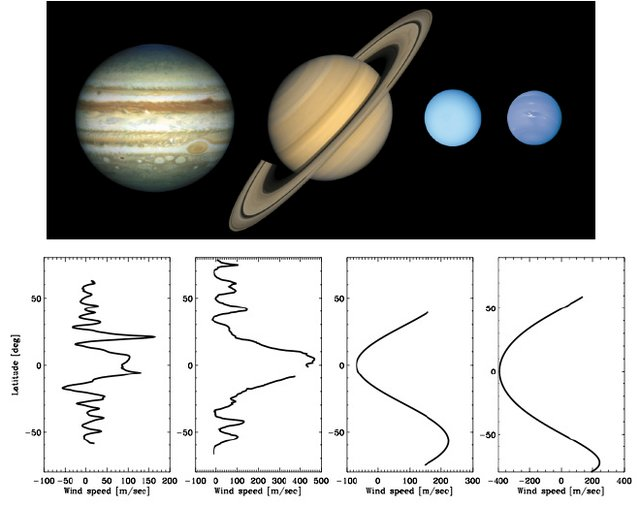
\includegraphics[clip,width=9cm]{./fig/intro/fig1.jpg}
    \caption{
      \footnotesize{上段 : 木星,土星,
天王星,海王星の可視光領域画像.
下段 : 縦軸が緯度,横軸が
クラウドトラッキングによって得られた
東西平均した東西風速分布.
巨大ガス惑星(木星,土星)は赤道域で幅の広い西風と
中緯度で東風/西風ジェットが交互に
約20個の帯状構造を形成しているのに対し,
巨大氷惑星(天王星,海王星)は
赤道域で幅の広い東風ジェットを含め
3つのジェットを形成している
\citep{showman2009atmospheric}.
      }
    }
    \label{fig1}
  \end{center}
\end{figure}
\clearpage
%
一方,極域の観測では
低中緯度ではあまり見られない空間スケールの大きい
低気圧性渦(自転と同じ向きに回転する渦)が
存在し,そのレジームが巨大惑星ごとに
異なることが近年のJuno, Cassini といった探査機の観測によって明らかになった.
%
図\ref{fig2} に木星と土星の極域観測を示した.
木星では複数の低気圧性渦が極付近にある低気圧性渦を
取り囲んでいるという特徴がある.
%
北極域では極から約$0.5^\circ$ 離れた位置に
低気圧性渦があり,その渦の周りを
8つの低気圧性渦が囲んでいる.
それぞれの渦の半径は約2000 - 2300 km (緯度幅で$\sim 2^\circ$) である.
%
南極域では極から約$1 \sim 2 ^\circ$ 離れた位置に
低気圧性渦があり,その渦の周りを
5つの低気圧性渦が囲んでいる.
それぞれの渦の半径は北極域のものより大きく,
約2800 - 3500 km (緯度幅で$\sim 3^\circ$) である\citep{Adriani2018}.

複数の低気圧性渦が存在する木星に対し,
土星では半径約2000 km (緯度幅で$\sim 2^\circ$) の
単一の低気圧性渦が各極域を支配している.
%
天王星,海王星もVoyger 2号と地上観測から
土星の低気圧性渦よりもサイズの大きい,
単一の低気圧性渦(緯度幅で$\sim 10^\circ$)が存在することが
示唆されている.
%
\begin{figure}[t]
  \begin{center}
    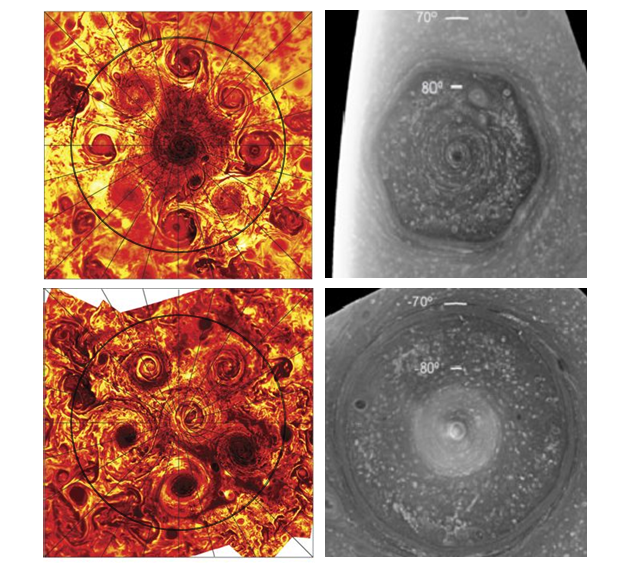
\includegraphics[clip,width=8cm]{./fig/intro/fig2.png}
    \caption{
      \footnotesize{左はJuno による木星観測(波長 : $5 \rm{\mu m}$).
黒の等緯度線は$80^\circ$ \citep{Adriani2018}.
右はCassini による土星観測(波長 : 750 nm) \citep{Antuano2015}.
上は北極域,下は南極域である.
      }
    }
    \label{fig2}
  \end{center}
\end{figure}
%
%
%\def\intro2{先行研究}
\section{先行研究}
\label{sec:intro2}
巨大惑星の内部構造の観測が難しいこともあり,
大気循環の力学的描像と理解は
数値計算を行い,\ref{sec:intro1}節で
述べた表層流の特徴の再現を通して,理解を試みてきた.
%
しかし,巨大惑星の内部構造は内部熱源があることなど,
地球型惑星の内部構造と大きく異なっており,
地球大気とのアナロジーで表層流を理解することは難しい.
特に,数値計算を行う際に問題になるのは
観測される表層の大気運動の深さである.
これについては大きく分けて,2つの説が考えられている.
%
1つは惑星内部の対流層と観測可能な雲が存在する大気上層部の
大気の運動が直接つながっているとする「深いモデル」である.
このモデルにおいては比較的,赤道域で強い西風ジェットは
形成されるものの,中高緯度域の帯状構造が発達しないという
問題点がある\citep{CHRISTENSEN2002}.
%
もう1つは,惑星深部の対流と大気上層部の対流は独立しており,
深部からの強制はあるものの深部の対流とは別のメカニズムで
構造が形作られているという「浅いモデル」である.
このモデルでは比較的,中高緯度の帯状構造が形成されるが,
赤道での西風ジェットが形成しないという問題点がある\citep{Scott2007}.
%
現在のところ決定的な議論は出来ていない.
%
%
\subsection{Showman et al. (2007)}
\label{sec:intro21}
これまでの「浅いモデル」の研究では
初期に小スケールの乱流を与え,時間発展をみる
自由減衰乱流実験\citep{Yoden1993}や
小規模な渦度強制を加える実験\citep{Scott2007}などが行われてきた.
%
しかし,このような全球的かつ連続的な
強制が巨大惑星に働いているとは考えにくい.
%
擾乱を引き起こす現象として
雷雲(\cite{Gierasch2000}, \cite{Porco2005}, \cite{Ingersoll2000})が考えられている.
%
\cite{Showman2007}はこの雷雲を想定した
局所的かつ離散的な強制を与え,球面浅水実験を行った.
彼らは緯度$0^\circ - 70^\circ$,経度$0^\circ - 120^\circ$の範囲の領域を計算した.
その結果,中緯度の変形半径が小さい場合($< 2000$ km) には図\ref{fig3} のように
帯状構造と赤道域で幅の広い東風ジェットが形成した.
計算した全てのケースで赤道では東風ジェットが形成した.
これは,減衰性乱流実験の結果と同様である\citep{Cho1996}.
また,中緯度では渦が支配的になることがわかった.
%
中緯度の変形半径が大きい場合($> 4000$ km) には,
弱い渦は伴うものの,ジェットが支配的にな
ことがわかった.
%
%
\begin{figure}[H]
  \begin{center}
    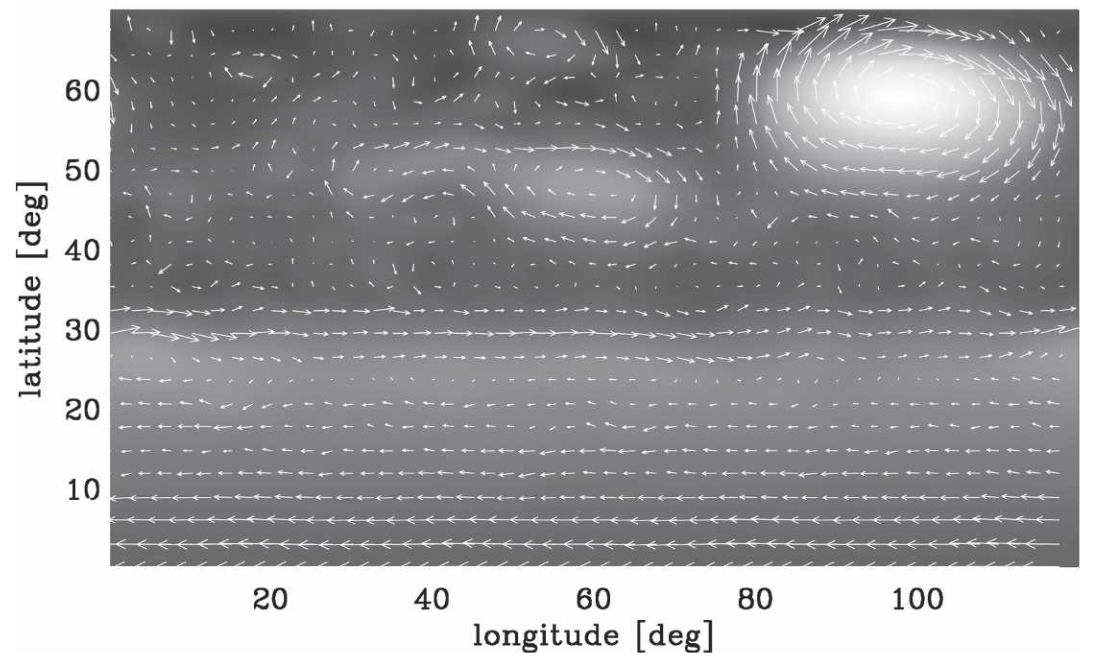
\includegraphics[clip,width=8cm]{./fig/intro/fig3.png}
    \caption{
      \footnotesize{ジオポテンシャルと
速度ベクトルの計算結果(4190地球日,中緯度の変形半径 : $L_d \sim 1200$ km).
トーン値の範囲は$0.21 : 2.7 \times 10^5 \rm{~m^2 \cdot s^{-2}}$.
速度の最大値は$96 \rm{~m \cdot s^{-1}}$.
\cite{Showman2007} Fig.1 より引用.
      }
    }
    \label{fig3}
  \end{center}
\end{figure}
%
\subsection{Brueshaber et al. (2019)}
\label{sec:intro22}
\cite{Brueshaber2019}は\cite{Showman2007}の雷雲を
想定した強制浅水実験を極域(約$\sim 60^\circ$ の等緯度線より高緯度)で計算し,
極渦とその数や大きさ,低気圧性・高気圧性といった特徴に注目した.
その結果,図\ref{fig4}に示すようにBurger 数(式(\ref{burger}))と呼ばれる
極での変形半径 : $L_{d0}$ と惑星半径 : $a$ の比で書かれる無次元量の値によって,
極渦の特徴が変化することがわかった.
%
Burger 数の値が$Bu \leq 2.40 \times 10^{-4}$の場合,
木星で観測されるような極のまわりを囲むような
配置は見られないが,複数の小さな低気圧性渦が形成する.
この特徴からこの特徴を木星的レジームと分類した.
%
Burger 数の値が$8.16 \times 10^{-4 } \leq Bu \leq  2.50 \times 10^{-3}$の場合,
土星で観測されるような極を中心とした単一の低気圧性渦が形成する.
この特徴からこの特徴を土星的レジームと分類した.
%
Burger 数の値が$4.00 \times 10^{-4 } \leq  Bu \leq  8.16 \times 10^{-4}$の場合,
高気圧性渦と低気圧性渦が混在する特徴があらわれる.
Burger 数が木星的レジームと土星的レジームの間にあるため
この特徴を遷移レジームと分類した.
%
Burger 数の値が$Bu \geq 4.44 \times 10^{-3 }$の場合,
土星的レジームよりも風速が大きい極を中心とした単一の低気圧性渦が形成する.
この特徴を氷巨大惑星的レジームと分類した.
%
\begin{figure}[H]
  \begin{center}
    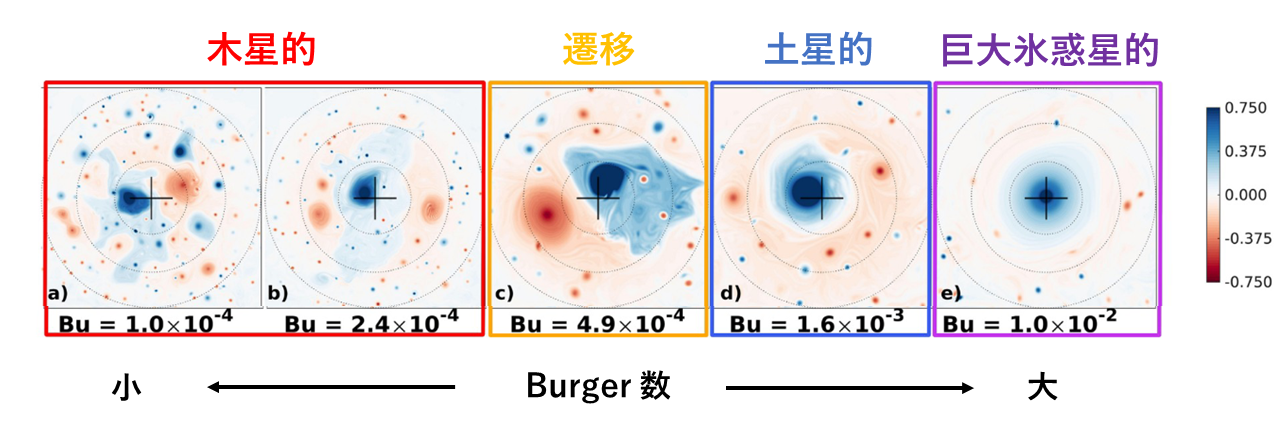
\includegraphics[clip,width=14cm]{./fig/intro/fig4_2.png}
    \caption{
      \footnotesize{無次元ポテンシャル渦度 : $Q_e^*$ (式(\ref{eq:nonqv}))の計算結果(20000地球日).
トーン値の範囲は$-0.75 : 0.75$.
上に\cite{Brueshaber2019}が分類した各レジーム名を示す.
Burger 数の値に応じて巨大惑星で観測されるような極渦の特徴が変化する.
$Q_e^* = 0$ は静止流体(相対渦度や流体層の厚さの水平平均からの変化はない),
北半球で $Q_e^* > 0$ は低気圧性渦,$Q_e^* < 0$ は高気圧性渦を表す.
\cite{Brueshaber2019} Fig.7 より引用.
      }
    }
    \label{fig4}
  \end{center}
\end{figure}
%
\def\intro3{研究目的}
\section{\intro3}
\label{sec:intro3}
雷雲を想定した強制を与えた浅水数値実験を
\cite{Showman2007}は低緯度から中緯度の領域を計算し,
赤道域のジェットと帯状構造に着目した.
境界条件としては,経度方向に周期境界,緯度方向はすべり境界 である.
%
一方,\cite{Brueshaber2019}は極域の領域で計算を行い,
極渦の特徴に着目した.
境界条件としては,周期境界だがスポンジ層により,流れは減衰する.
%
どちらの先行研究も領域計算であり,
全球計算を行い,彼らの結果を確かめる必要がある.
なぜなら,先行研究では考慮されていない計算領域外からの運動量輸送などにより,
計算で得られたジェットや渦の構造が変化する可能性があるからである.
%
%
%例えば,\cite{Heimpel2007}は薄い球殻領域内の
%深部対流運動を全球の1/8 の領域で解き,
%帯状構造と赤道加速が共存する状態を数値的に再現した.
%しかし,この計算を全球で計算した
%\cite{Takehiro2015}では時間積分を進めると帯状構造が
%消滅するという結果がある.
%
そのため本研究では,雷雲を想定した
強制浅水実験を全球で行い,
観測されている帯状構造と渦構造が
雷雲による強制により,形成されるのかを調べる.
%
また,それらの構造を
\cite{Showman2007}, \cite{Brueshaber2019} の結果と比較し,
彼らの領域計算で得られた結果の妥当性を調べる.
%
\def\intro4{本論文の構成}
\section{\intro4}
\label{sec:intro4}
本論文の構成を簡単に述べる.
\ref{chap:2}章では用いた1.5層浅水方程式系と
数値実験の手法および設定について述べる.
\ref{chap:3}章ではBurger 数,放射緩和時間,
低気圧性渦/高気圧性渦の割合,解像度のそれぞれの
値を変化させたときの実験結果を示す.
\ref{chap:4}章では
帯状構造と極渦の構造に注目し議論とまとめを行う.
%\ref{chap:5}章で本論文の結論を述べる.
%
%
\setcounter{table}{0}
\def\chap2{モデルと手法}
\chapter{\chap2}
\label{chap:2}
\markright{2 \chap2}
ここでは本研究で用いるモデルと実験手法・実験設定について述べる.
\section{支配方程式系}
\label{sec:model1}
本研究では球面上の1.5層浅水方程式系を用いる.
これは\cite{Showman2007}, \cite{Brueshaber2019}で用いられた系と同じである.
このモデルにおいて上層と下層はそれぞれの層で密度一定であり,
上層は活動的な層,下層は無限に深く静止した層であると仮定する.
上層に対する運動量方程式と質量保存の式は
%
\begin{align}
& \DD{\Dvect{u}}{t}+ g' \Dgrad h + f \Dvect{k} \times \Dvect{u} = -\Dvect{D}_{\Dvect{u}},  \label{eq:eq1} \\
& \DP{g'h}{t} + \Ddiv (g'h\Dvect{u}) = \Sigma S_{{\rm{storm}}} + S_{{\rm{rad}}} - D_h \label{eq:eq2} 
\end{align}
%
である\footnote{導出は付録 \ref{ape:A}を参照.}.
$\Dvect{u}$は水平風速,$g'$は有効重力加速度,
$h$は上層の厚さ,$f$はコリオリパラメータ,
$\Dvect{k}$は鉛直方向の単位ベクトル,
$\Dvect{D}_u, D_h$はそれぞれ計算が
発散しないための数値粘性・拡散項\footnote{詳細は付録\ref{ape:B}を参照.},
$S_{{\rm{storm}}}$は雷雲を想定した質量強制項,$S_{{\rm{rad}}}$ は放射緩和項である.
また,物質微分は
\begin{align}
\DD{}{t} = \DP{}{t} + \frac{u}{a\cos{\vartheta}} \DP{}{\lambda}
+\frac{v}{a} \DP{}{\vartheta}.
\end{align}
それぞれの強制項は
\begin{align}
&S_{{\rm{storm}}} = s \cdot \exp \left [- \frac{R^2}{R_{{\rm{storm}}}^2} - \frac{(t^*-t_0)^2}{\tau_{{\rm{storm}}}^2} \right ], \label{eq:eq3}\\
&S_{{\rm{rad}}}  = - \frac{\langle g'h \rangle - g'h_{{\rm{eq}}}}{\tau_{{\rm{mass}}}} - \frac{g'h - \langle g'h \rangle}{\tau_{{\rm{APE}}}} \label{eq:eq4}
\end{align}
である.
%
ここで,$s$は質量強制の最大値,
またその正負の割合を$\alpha$とする.
$\alpha=1.0$ のとき,正の質量強制のみが与えられる
(つまり,高気圧性渦が質量強制を与えた領域で発生する).
$R$は質量強制の中心位置からの距離,
$R_{{\rm{storm}}}$は質量強制の半径,
$t^*$は質量強制が局所的に与えられてからの時間,
$t_0$は質量強制がピークを迎える時間,
$\tau_{{\rm{storm}}}$は質量強制の特徴的な緩和時間,
$\langle \rangle$ はその瞬間の水平平均,
$h_{{\rm{eq}}}$は平衡状態での厚さ,
$\tau_{{\rm{mass}}}$はエネルギーに影響を与えず,
$\langle g'h \rangle $を$g'h_{{\rm{eq}}}$に向かって平衡化するときの緩和時間,
$\tau_{{\rm{APE}}}$は質量に影響を与えず,
$g'h$を$\langle g'h \rangle$に向かって平衡化するときの緩和時間である.
図\ref{fig5}に質量強制のスナップショットを示す.
%
\begin{figure}[t]
  \begin{center}
    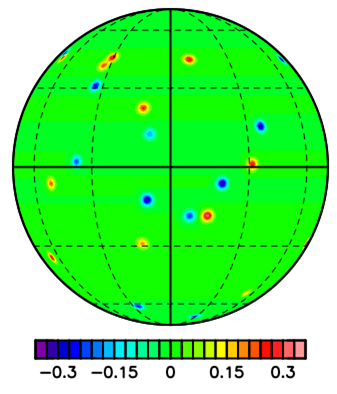
\includegraphics[clip,width=6cm]{./fig/model/fig5_v2.png}
    \caption{
      \footnotesize{質量強制 : $S_{{\rm{storm}}}$ のスナップショット($s_{max} = 0.333$, $R_{{\rm{storm}}} = 2.62 \times 10^6 {\rm{~m~}}(2.1^{\circ})$
, $\alpha = 0.5$の場合).
ある時刻と位置に雷雲を想定した質量強制を式(\ref{eq:eq3})で与える.
質量強制は$R > 2.2 R_{{\rm{storm}}}, t^* > 2.2 \tau_{{\rm{storm}}}$ で0とする.
質量強制が与えられてから,$2.2 \tau_{{\rm{storm}}}$ 秒後に消滅.
そこから$\tau_{{\rm{interval}}}$ 秒後に違う位置に質量強制が与えられる.
      }
    }
    \label{fig5}
  \end{center}
\end{figure}
%
質量強制は$R > 2.2 R_{{\rm{storm}}}, t^* > 2.2 \tau_{{\rm{storm}}}$ で0 とする.
質量強制が与えられてから,$2.2 \tau_{{\rm{storm}}}$ 秒が経過し,消滅後,
そこから$\tau_{{\rm{interval}}}$ 秒後に違う位置に質量強制が与えられる.

式(\ref{eq:eq4}) の放射緩和項の右辺第1項は
緩和時間$\tau_{{\rm{mass}}}$ で$\langle g'h \rangle $を
平衡厚さ$g'h_{{\rm{eq}}}$に向かって,緩和する.
%
右辺第2項は緩和時間$\tau_{{\rm{APE}}}$ で
局所的な$g'h$を$\langle g'h \rangle $に向かって,緩和する.
%
これは物理的には潜熱を放出する雷雲のような大気の暖かい領域が
冷たい領域よりも早く冷えるという効果をあらわしている.
%
これら2つの項により,統計的定常状態を実現する.
%
\cite{Brueshaber2019} ではこれらの強制項に加え,質量強制による質量の増減を
調整する質量調整項を加えていたが,
ここでは\cite{Showman2007}にならい,加えない.
使用する記号を表\ref{table:para}にまとめる.
\begin{table}[t]
  \caption{本論文中で使用する記号一覧}
  \label{table:para}
  \begin{center}
    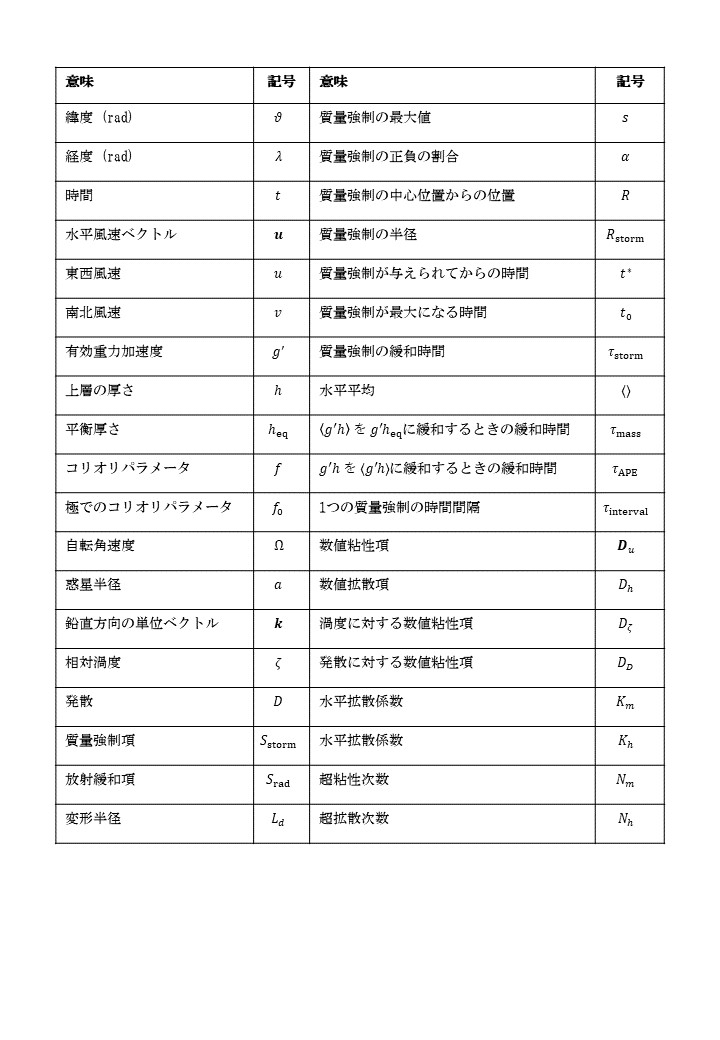
\includegraphics[clip,width=15cm]{./fig/model/table_para-2.jpg}
  \end{center}
\end{table}
%
\clearpage
\newpage
\section{実験手法・実験設定}
\label{sec:model2}
1.5層球面浅水系の方程式(\ref{eq:eq1}), (\ref{eq:eq2}) を解く.
その際,運動量方程式はベクトル量である速度のままだと
球面座標系では格子点が集中する極点付近で,計算が難しい.
そのため,式(\ref{eq:eq1})を変形しスカラー量である渦度と発散に関する式を用いる\footnote{付録 \ref{ape:B} を参照.}.
%
また,数値的な安定性を維持するために
ラプラシアン4次の超粘性を加える.
%
空間離散化にはスペクトル法を用いる.
時間離散化は数値粘性項についてはクランク・ニコルソン法,
それ以外の項には4次のルンゲクッタ法を用いる.
%
数値モデルの作成には地球流体電脳倶楽部の階層的地球スペクトルモデル集
(SPMODEL; \cite{spmodel2006}, \cite{spmodel2013}) を使用する.
また,スキームの確認と並列化効率の測定のために
\cite{Williamson1992} が提案したテストセットを
実行した\footnote{付録\ref{Williamson}を参照.}.

初期に上層は静止しており,$10 \tau_{{\rm{interval}}}$ 秒経過する間に
最初の質量強制がランダムな位置に最大で50個加えられる.
%
自転角速度は木星の値を用いる.
また,計算時間は3000 地球日とする.
%
本研究で用いた共通パラメータを表\ref{table1} に示す.
表\ref{table2}に計算を行った数値実験のケースとその用いたパラメータを示す.

以下ではA1 のケースを標準実験とし,\ref{sec:A1}節でその実験結果について述べる.
%
その次に,\ref{sec:case1}節では$g'h_{{\rm{eq}}}$,または$a$を変化させ,Burger 数の影響を調べた実験1の結果について示す.
\ref{sec:case2}節では$\tau_{{\rm{APE}}}$の値を変化させ,放射緩和項の緩和時間の影響を調べた実験2の結果について示す.
\ref{sec:case3}節では$\alpha$の値を変化させ,質量強制の正負の影響を調べた実験3の結果について示す.
\ref{sec:case4}節では解像度をかえ,質量強制の空間的大きさの影響を調べた実験4の結果について示す.
それぞれの実験について,表\ref{table:exp}にまとめる.
\begin{table}[ht]
  \caption{実験で用いた共通パラメータ}
  \label{table1}
  \begin{center}
    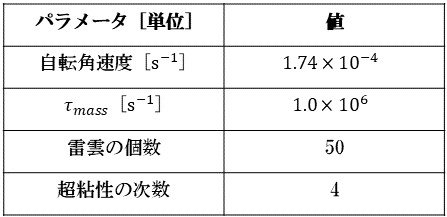
\includegraphics[clip,width=8cm]{./fig/model/table1.jpg}
  \end{center}
\end{table}
%
%
\newpage
\begin{landscape}
\begin{table}[t]
  \caption{実験のケースと用いたパラメータ}
  \label{table2}
  \begin{center}
    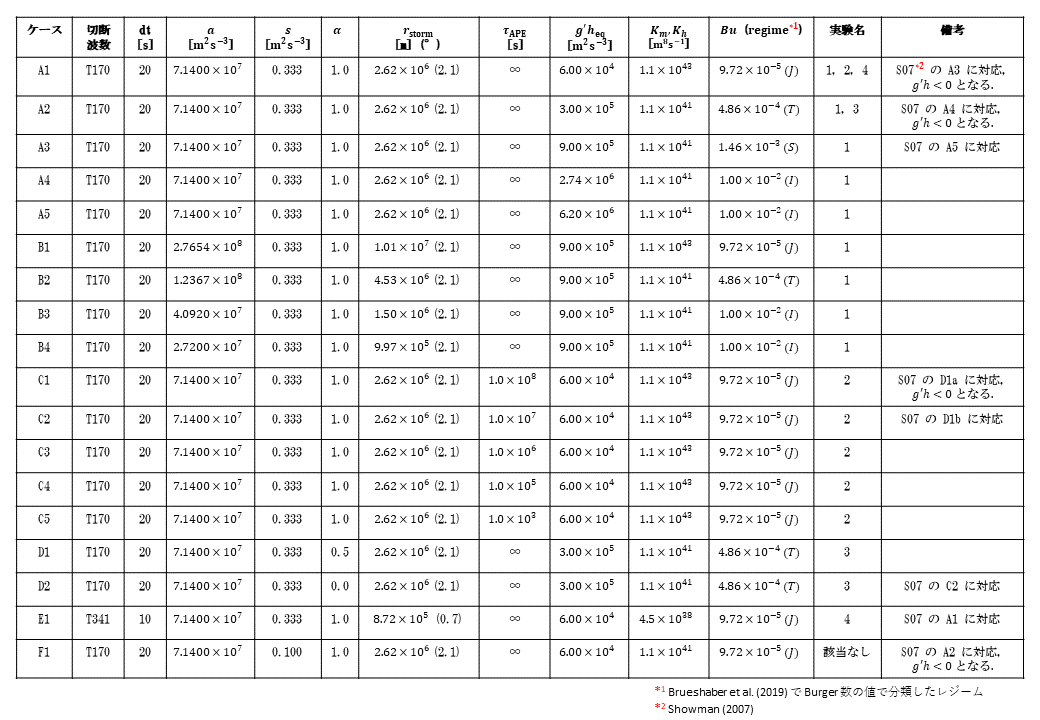
\includegraphics[clip,width=20cm]{./fig/model/table2_v2.png}
  \end{center}
\end{table}
\end{landscape}
%
\begin{table}[ht]
  \caption{各実験の説明}
  \label{table:exp}
  \begin{center}
    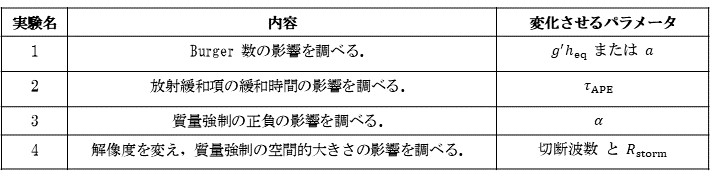
\includegraphics[clip,width=14cm]{./fig/model/table_exp.jpg}
  \end{center}
\end{table}
%
\clearpage
\def\chap3{実験結果}
\chapter{\chap3}
\label{chap:3}
\markright{3 \chap3}
%
%%%%%%%%%%%%%%%%%% 標準実験 : A1 %%%%%%%%%%%%%%%%%%%
\section{標準実験結果 : A1}
\label{sec:A1}
この節では,標準実験とした A1 のケースの結果を図\ref{fig:A1_1}-\ref{fig:A1_5}に示す.
用いたパラメータは表\ref{table2}を参照.
図\ref{fig:A1_1}の東西風速を見てわかるように,
赤道域で幅が広く,風速が約$220 \rm{~m \cdot s^{-1}}$と強力な東風ジェットと
緯度約$\pm 30^\circ$ で風速約$100 \rm{~m \cdot s^{-1}}$の西風ジェットが見られる.
%
また,その西風ジェットに対応して,図\ref{fig:A1_2}のジオポテンシャルが
その領域で値が大きくなっている.
%
正(負)の質量強制の場合,流体層に局所的な膨らみ(窪み)を作る.
この膨らみ(窪み)はコリオリ力により,高気圧性(低気圧性)渦を形成する.
%
このケースでは正の質量強制のみ与えられるため,
図\ref{fig:A1_3}を見て分かるように,
高気圧性渦が見られる.
%
また,ポテンシャル渦度はほぼラグランジュ的に保存するため,流体の性質を見るために役立つ.
\cite{Brueshaber2019} では背景場のポテンシャル渦度からの
渦の性質を知るために,次の無次元ポテンシャル渦度 : $Q_e^*$ を定義した.
\begin{align}
Q_e^* = \left [\frac{\zeta+f}{h}-\frac{f}{\langle h \rangle}\right]\cdot \frac{\langle h \rangle}{f_0}. \label{eq:nonqv}
\end{align}
ここで,$\zeta$は相対渦度,$f$はコリオリパラメータ,$f_0$は極でのコリオリパラメータの値である.
%
$Q_e^*=0$は静止流体(相対的な渦度や厚さの摂動はない)を表す.
北半球で $Q_e^*>0$は低気圧性の渦度を表し,
$Q_e^*<0$は高気圧性の渦度を表す.
%
図\ref{fig:A1_4}の極域を見てみると巨大な低気圧性渦の中に,複数の高気圧性渦が形成していることがわかる.
%
図\ref{fig:A1_5}に有効ポテンシャルエネルギー : APE と運動エネルギー : KE 
\begin{align}
APE &= \frac{1}{2} \int \left[(g'h)^2 - \langle g'h \rangle^2   \right] dA. \label{eq:APE} \\
KE  &= \frac{1}{2} \int g'h(u^2 + v^2) dA. \label{eq:KE}
\end{align}
を示す.ここで,$A$ は計算領域の面積,$u, v$ はそれぞれ経度,緯度方向の速度である.
%
A1 のケースでは$\tau_{{\rm{APE}}} = \infty$ のため,局所的な緩和が効かず,APE とKE は時間とともに増加する.
このケースは\cite{Showman2007}のA3 のケースに対応するが,
極域でジオポテンシャルが負になる領域があることがわかった(他のケースについては表\ref{table2} 備考を参照.).
この系の上端の境界条件は剛体表面なので,物理的にはありえない. % 物理的にはありえないと書いてはいけない
\cite{Showman2007} が用いた$g'h_{\rm{eq}}$の値によっては,
そのような数値解が得られてしまうことがわかった\footnote{A1のケースでは... この文は修正が必要.
$g'h$が負になった場合に,描画しているものは何なのかを説明する. }.
%
\begin{figure}[b]
  \begin{center}
    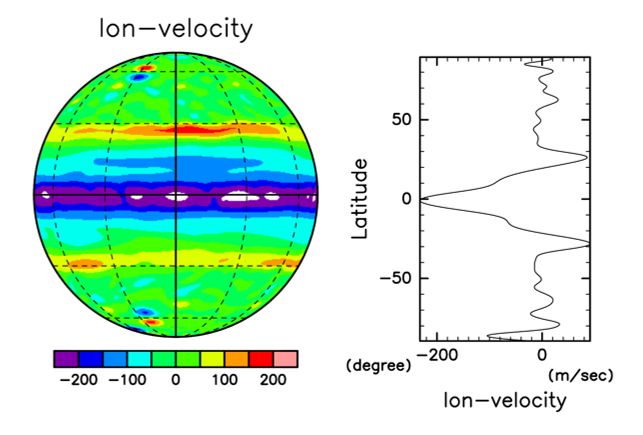
\includegraphics[clip,width=10cm]{./fig/result/A1/A1_1.png}
    \caption{
      \footnotesize{A1の実験結果. 左 : 緯度$0^\circ$,経度$0^\circ$から見た球面投影の東西風速,右 : 東西平均した東西風速(3000 地球日).
      }
    }
    \label{fig:A1_1}
  \end{center}
\end{figure}
%
\begin{figure}[ht]
  \begin{center}
    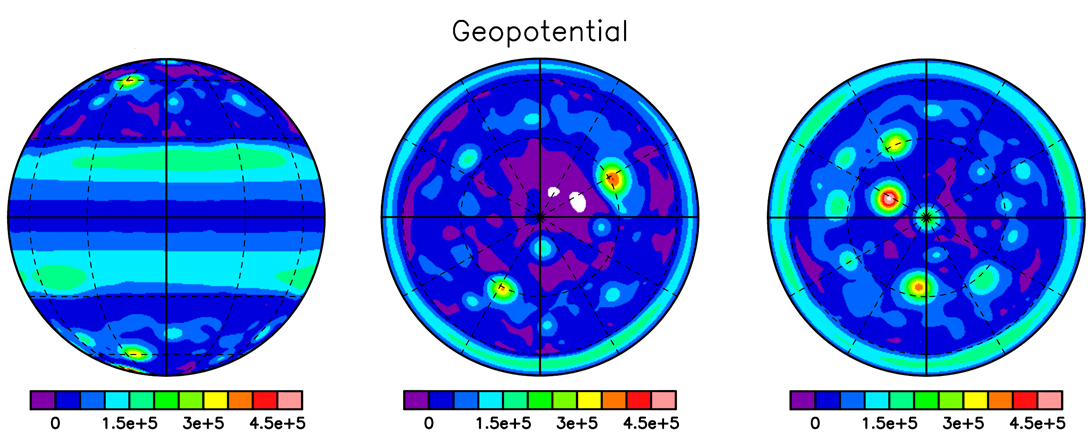
\includegraphics[clip,width=12cm]{./fig/result/A1/A1_2.png}
    \caption{
      \footnotesize{A1の実験結果. ジオポテンシャル(3000 地球日).
左 : 緯度$0^\circ$,経度$0^\circ$から見た球面投影.
中 : 緯度$90^\circ$ から見た球面投影.
右 : 緯度$-90^\circ$ から見た球面投影.
      }
    }
    \label{fig:A1_2}
  \end{center}
\end{figure}
%
\begin{figure}[ht]
  \begin{center}
    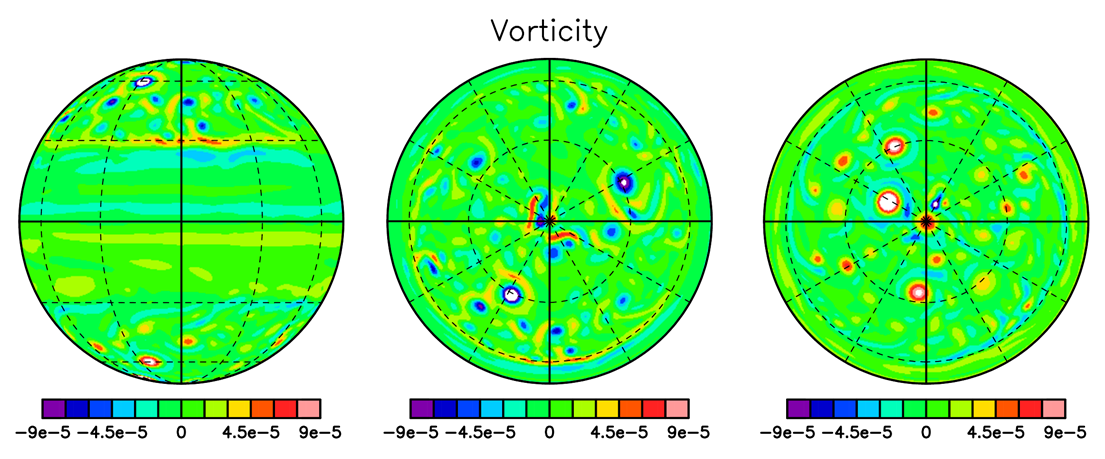
\includegraphics[clip,width=12cm]{./fig/result/A1/A1_3.png}
    \caption{
      \footnotesize{A1の実験結果. 相対渦度(3000 地球日).
左 : 緯度$0^\circ$,経度$0^\circ$から見た球面投影.
中 : 緯度$90^\circ$ から見た球面投影.
右 : 緯度$-90^\circ$ から見た球面投影.
      }
    }
    \label{fig:A1_3}
  \end{center}
\end{figure}
%
\begin{figure}[ht]
  \begin{center}
    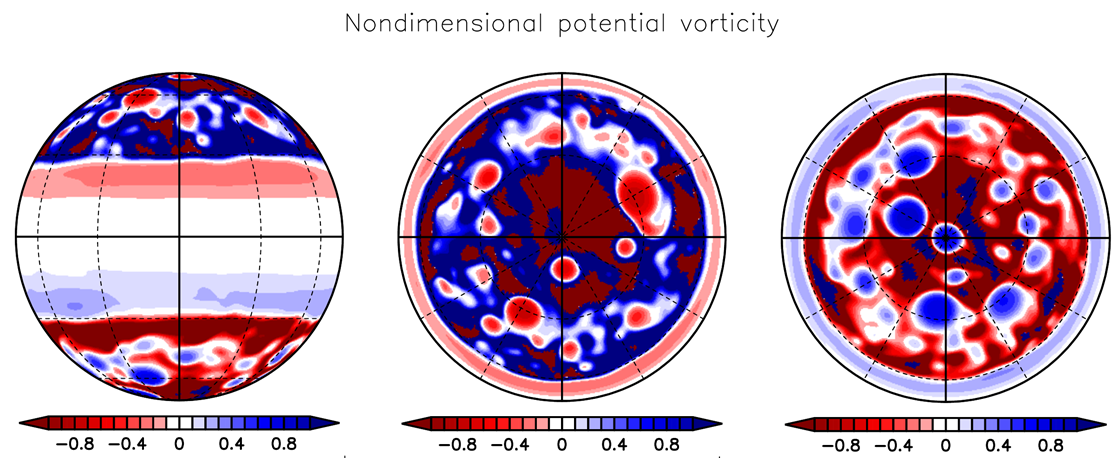
\includegraphics[clip,width=12cm]{./fig/result/A1/A1_4.png}
    \caption{
      \footnotesize{A1の実験結果. 無次元ポテンシャル渦度(3000 地球日).
左 : 緯度$0^\circ$,経度$0^\circ$から見た球面投影.
中 : 緯度$90^\circ$ から見た球面投影.
右 : 緯度$-90^\circ$ から見た球面投影.
無次元ポテンシャル渦度のトーン値の範囲は$-1:1$である.
      }
    }
    \label{fig:A1_4}
  \end{center}
\end{figure}
%
\begin{figure}[ht]
  \begin{center}
    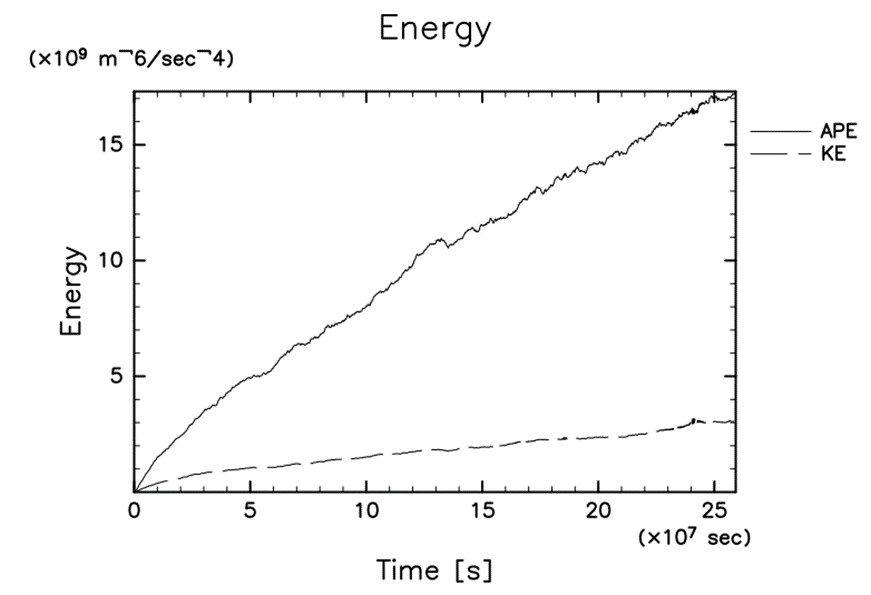
\includegraphics[clip,width=12cm]{./fig/result/A1/A1_5.jpg}
    \caption{
      \footnotesize{A1の実験結果. 有効ポテンシャルエネルギー : APE (実線) と運動エネルギー : KE (点線) の時間発展.
      }
    }
    \label{fig:A1_5}
  \end{center}
\end{figure}
%
%%%%%%%%%%%%%%%%%% case1 : Burger %%%%%%%%%%%%%%%%%%%
\clearpage
\newpage
\section{実験1 : Burger 数の変化による影響}
\label{sec:case1}
この節ではBurger 数 
\begin{align}
Bu = \left (\frac{L_{d0}}{a} \right )^2 \label{burger}
\end{align}
の変化による影響を調べる.
$a$は惑星半径,$L_{d0}$は極での変形半径
\begin{align}
L_{d0} = \frac{\sqrt{g'h_{{\rm{eq}}}}}{f_0}, \qquad f_0 = 2 \Omega
\end{align}
である.\cite{Brueshaber2019}ではBurger 数を初期の値から
変化しないように,質量強制によって加えられた質量を
全球の流体層の厚さから取り除く項を入れているが,
本研究では平衡厚さ$g'h_{{\rm{eq}}}$でBurger 数を定義する.

%
図\ref{fig:case1_nonqv_a}に$a$を
図\ref{fig:case1_nonqv_gh}に$g'h_{\rm{eq}}$を変化させた実験の
無次元ポテンシャル渦度を示す.
%
図の下に示されているアルファベットは\cite{Brueshaber2019}が
Burger 数によって,分類した極渦のレジームを示している.
表\ref{table:regime} に\cite{Brueshaber2019}が分類した極渦のレジームの特徴と
そのBurger 数の値の範囲を示す.
%

結果(仮)
%%%%%%%%%%%%%%%%%%%%%%%%
\begin{itemize}
\item{Burger 数の値によって,極渦のレジームが異なる.}
\item{風速分布は$Bu \leq 1.46 \times 10^{-3} $ で
赤道域で東風ジェット,中緯度域では帯状構造と
緯度約$\pm 20^\circ - 30^\circ$で西風ジェットが形成.
\cite{Showman2007} に比べ,赤道域のジェットの風速が大きい.}
\end{itemize}
%

文章(仮) 

図\ref{fig:case1_nonqv_a}, 図\ref{fig:case1_nonqv_gh} を見て分かるように,
B1, A1 ($Bu = 9.72\times 10^{-5}$) では,
複数の高気圧性渦が見られる.
これは\cite{Brueshaber2019} の木星的レジームに対応し,
その特徴と一致している.
%
B2, A2 ($Bu = 4.86\times 10^{-4}$) は
遷移レジームに対応し,
A2 は比較的大きい高気圧性渦と低気圧性渦が混在するが,B2 はその特徴が見られない.
%
A3 ($Bu = 1.46\times 10^{-3}$) は
土星的レジームに対応し,
極中心に単一の低気圧性渦が形成する.
%
B3, A4 ($Bu = 4.44 \times 10^{-3}$), 
B4, A5 ($Bu = 1.00 \times 10^{-2}$) は
巨大氷惑星的レジームに対応する.
A5 を除き,土星的レジームと同様, 
極中心に単一の低気圧性渦が形成する.
この低気圧性渦による極域の風速は
図\ref{fig:case1_vellon_a}, 図\ref{fig:case1_vellon_gh} を
見て分かるように低緯度の風速に比べて大きい.
これは巨大氷惑星的レジームの特徴であり,
\cite{Brueshaber2019} の結果と一致している\footnote{整合的であると言え.}.
%

東西風分布を見てみると,
$Bu \leq 1.46 \times 10^{-3} $  の場合で,
赤道域の東風ジェット,中緯度域では帯状構造と
緯度約$\pm 20 - 30^\circ$で西風ジェットが形成している.
また風速は$Bu$ が大きくなるにつれて,小さくなる.
%
\cite{Showman2007} との東西風分布の比較を図\ref{fig:case1_rms_comp} に示す.
\cite{Showman2007} と比較して,我々の計算では
赤道域の東風ジェットの風速が大きい.
これは,\cite{Showman2007} では領域計算のため,
考慮出来なかった南半球からのエネルギー輸送が要因のひとつとして考えられる
\footnote{本当に? 議論で説明する.}.
% 

%%%%%%%%%%%%%%%%%%%%%%%%
%
\begin{table}[h]
  \caption{極渦のレジームの分類とその特徴}
  \label{table:regime}
  \begin{center}
    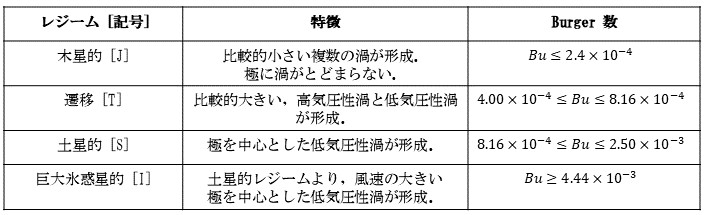
\includegraphics[clip,width=15cm]{./fig/model/table_regime.jpg}
  \end{center}
\end{table}
%
\begin{figure}[ht]
  \begin{center}
    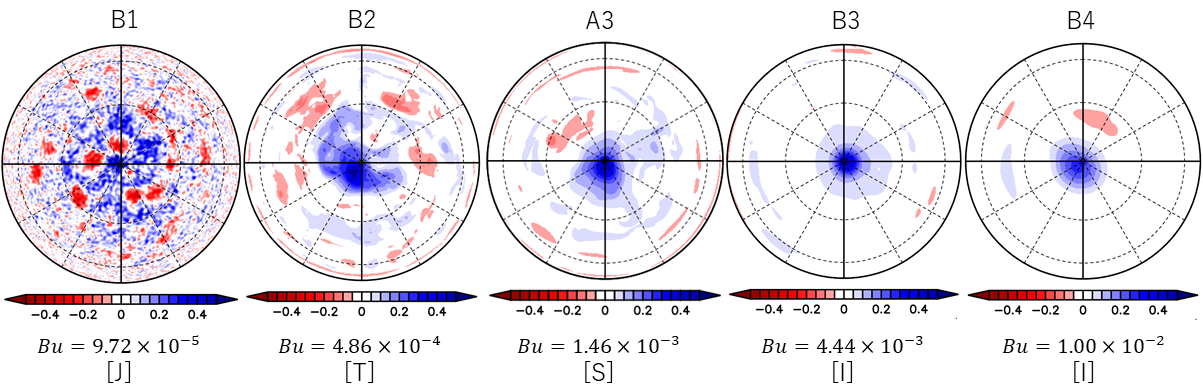
\includegraphics[clip,width=14cm]{./fig/result/case1/case1_nonqv_a.png}
    \caption{
      \footnotesize{緯度$90^\circ$ から見た球面投影の無次元ポテンシャル渦度(3000 地球日).
上にケース名,下にBurger 数と\cite{Brueshaber2019}で分類された極渦のレジームを示している.
$a$ を変化させ,Burger 数の値をかえた.
無次元ポテンシャル渦度のトーン値の範囲は$-0.5:0.5$である.
      }
    }
    \label{fig:case1_nonqv_a}
  \end{center}
\end{figure}
%
\begin{figure}[ht]
  \begin{center}
    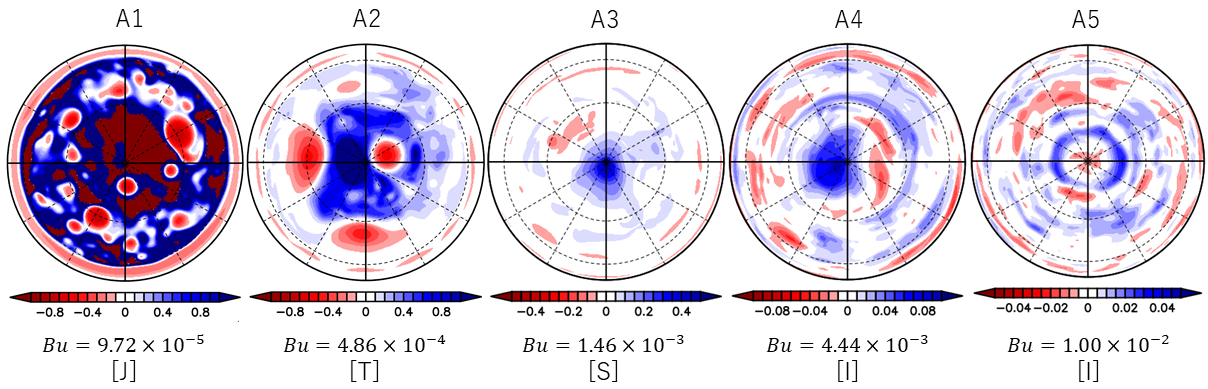
\includegraphics[clip,width=14cm]{./fig/result/case1/case1_nonqv_gh.png}
    \caption{
      \footnotesize{緯度$90^\circ$ から見た球面投影の無次元ポテンシャル渦度(3000 地球日).
上にケース名,下にBurger 数と\cite{Brueshaber2019}で分類された極渦のレジームを示している.
$g'h_{\rm{eq}}$ を変化させ,Burger 数の値をかえた.
無次元ポテンシャル渦度のトーン値の範囲は左から,$-1:1, -1:1, -0.5:0.5, -0.1:0.1, -0.05:0.05$である.
      }
    }
    \label{fig:case1_nonqv_gh}
  \end{center}
\end{figure}
%
\clearpage
\newpage
%
\begin{figure}[ht]
  \begin{center}
    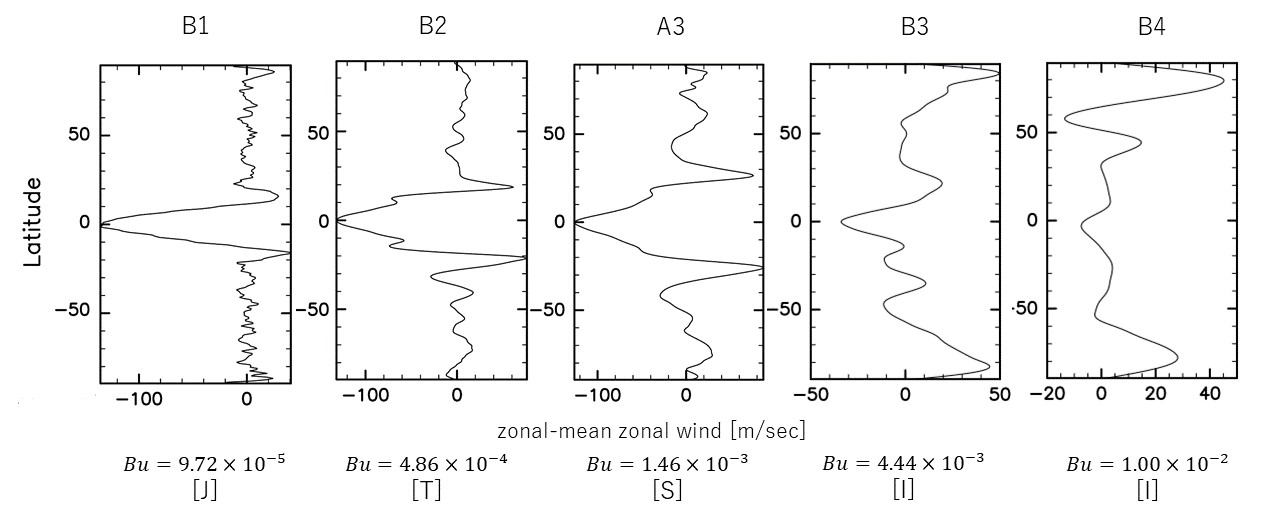
\includegraphics[clip,width=14cm]{./fig/result/case1/case1_vellon_a.jpg}
    \caption{
      \footnotesize{東西平均した東西風速(3000 地球日).
上にケース名,下にBurger 数と\cite{Brueshaber2019}で分類された極渦のレジームを示している.
$a$ を変化させ,Burger 数の値をかえた.
      }
    }
    \label{fig:case1_vellon_a}
  \end{center}
\end{figure}
%
%
\begin{figure}[ht]
  \begin{center}
    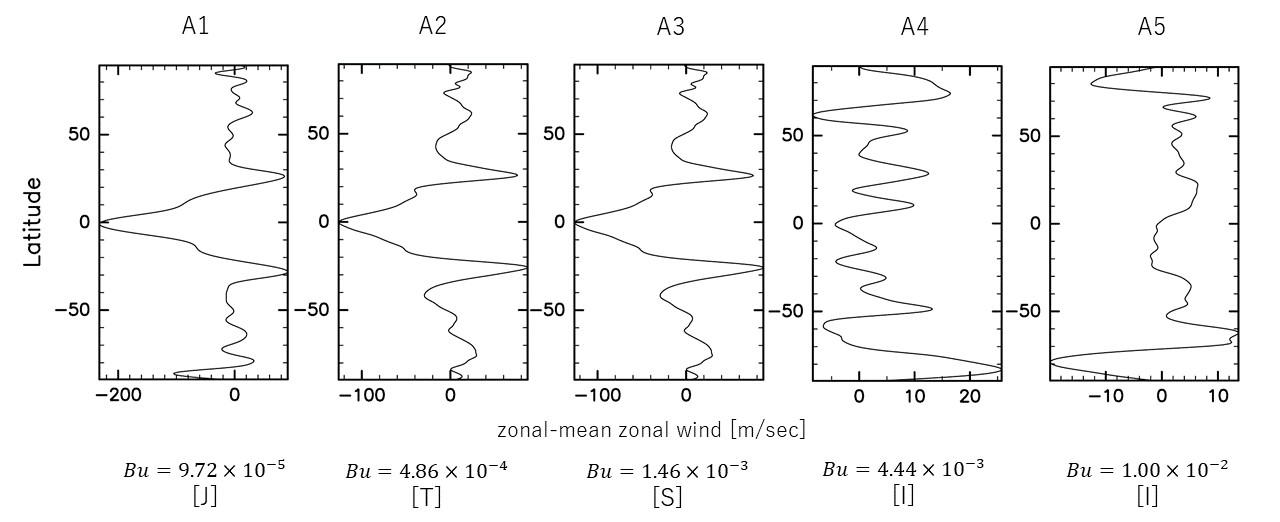
\includegraphics[clip,width=14cm]{./fig/result/case1/case1_vellon_gh.jpg}
    \caption{
      \footnotesize{東西平均した東西風速(3000 地球日).
上にケース名,下にBurger 数と\cite{Brueshaber2019}で分類された極渦のレジームを示している.
$g'h_{\rm{eq}}$ を変化させ,Burger 数の値をかえた.
      }
    }
    \label{fig:case1_vellon_gh}
  \end{center}
\end{figure}
%
\begin{figure}[ht]
  \begin{center}
    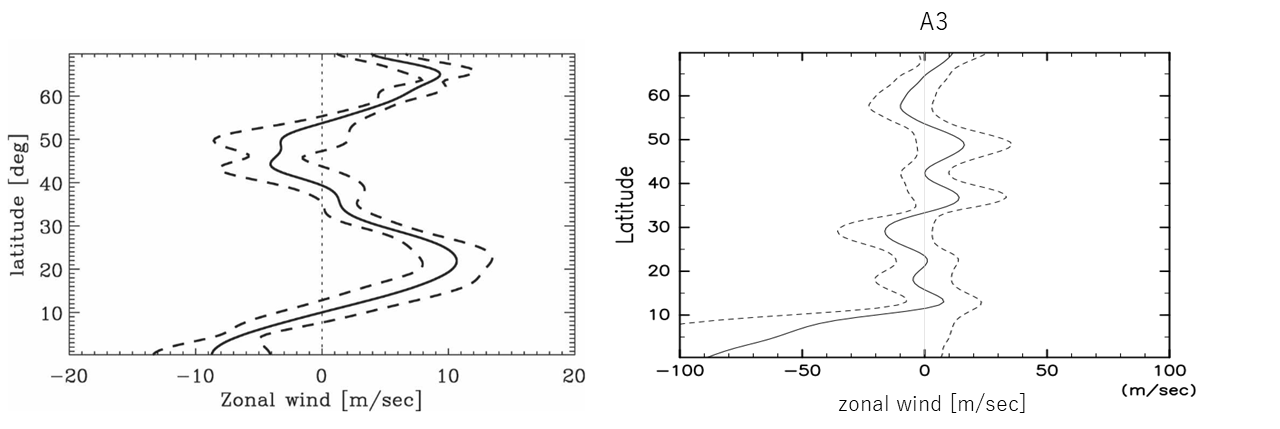
\includegraphics[clip,width=14cm]{./fig/result/case1/case1_rms_comp.png}
    \caption{
      \footnotesize{東西平均した東西風速の比較(2200 地球日).
左 : \cite{Showman2007} の結果(彼らのFig. 5 より引用).
右 : 計算結果.
実線は東西平均した東西風速,破線は二乗平均速度との差.
      }
    }
    \label{fig:case1_rms_comp}
  \end{center}
\end{figure}
%
%
%%%%%%%%%%%%%%%%%% case2 : tau_APE %%%%%%%%%%%%%%%%%%%
\clearpage
\newpage
\section{実験2 : $\tau_{\rm{APE}}$ の変化による影響}
\label{sec:case2}
この節では放射緩和項の$\tau_{\rm{APE}}$の変化による影響を調べる.
$\tau_{\rm{APE}}$は$g'h$を$\langle g'h \rangle $ に向かって緩和する.
行ったケースは$\tau_{\rm{APE}} = \infty, 10^8, 10^7, 10^6, 10^5, 10^3$ である.
図\ref{fig:case2_nonqv},図\ref{fig:case2_vellon} に

結果(仮)
%%%%%%%%%%%%%%%%%%%%%%%%
\begin{itemize}
\item{$\tau_{\rm{APE}}$の値が小さくなるにつれて,極渦,ジオポテンシャルの
空間スケールが小さくなる.}
\item{$\tau_{\rm{APE}}$の値が小さくなるにつれて,風速が弱くなる.
赤道域でジェットが形成する場合,東風となる.}
\end{itemize}
%

文章(仮) 

図\ref{fig:case2_nonqv},\ref{fig:case2_phi1},\ref{fig:case2_phi2} に
無次元ポテンシャル渦度とジオポテンシャルを示す.
%
$\tau_{\rm{APE}}$ の値が小さくなるに従い,
局所的な緩和が効くため,質量強制が
与えられた領域の$g'h$ が $\langle g'h \rangle$に向かってすぐさま緩和する.
そのため,実験\ref{sec:case1}で見られたような特徴的な極渦や
空間スケールの大きい渦が現れない.
特に,C4, C5 のケースではほとんど,強制の影響がみられない.
%
これは,質量強制による小スケールのエネルギーが
逆カスケードする前に緩和が効き,エネルギーが取り除かれ,
結果的に空間スケールの小さい構造が形成すると考えられる.
%
図\ref{fig:case2_vellon} の東西平均した東西風速も
$\tau_{\rm{APE}}$の値が小さくなるに従い,
風速が小さくなり,C4, C5 のケースでほとんど0となる.
赤道域のジェットが形成する場合,\ref{sec:case1} 節と同様,東風となる.
%

APE(式(\ref{eq:APE})) とKE(式(\ref{eq:KE})) の値を図\ref{fig:case2_apeke} に示す.
$\tau_{\rm{APE}}=\infty$ の A1 のケースでは,APE とKE は時間とともに増加していくが
(縦軸に対数をとっていない図は\ref{sec:A1}節の図\ref{fig:A1_5}を参照.),
$\tau_{\rm{APE}}$が有限値の場合,ある時間でエネルギーの注入率と除去率が
平衡し,一定の値付近で振動することがわかる.
また,計算をはじめてからエネルギーが
平衡化するまでの時間は$\tau_{\rm{APE}}$が小さくなるにつれて,みじかくなる.
%
\begin{figure}[ht]
  \begin{center}
    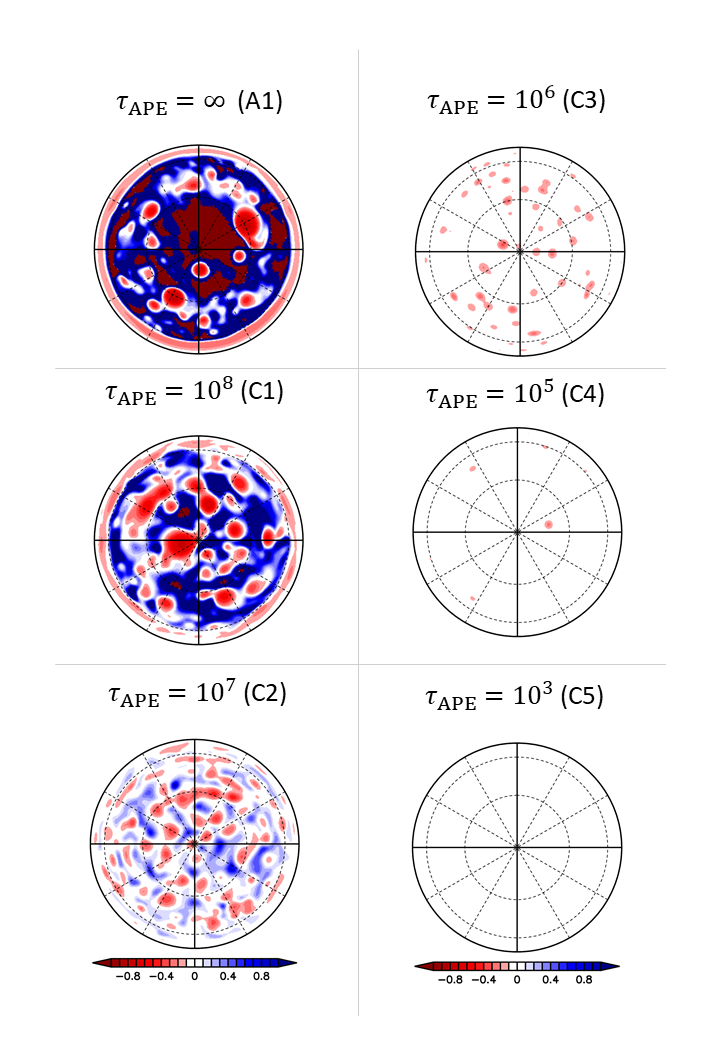
\includegraphics[clip,width=14cm]{./fig/result/case2/case2_nonqv.png}
    \caption{
      \footnotesize{緯度$90^\circ$ から見た球面投影の無次元ポテンシャル渦度(3000 地球日).
上に$\tau_{\rm{APE}}$ の値とケース名を示す.
無次元ポテンシャル渦度のトーン値の範囲は$-1:1$である.
      }
    }
    \label{fig:case2_nonqv}
  \end{center}
\end{figure}
%
%
\begin{figure}[ht]
  \begin{center}
    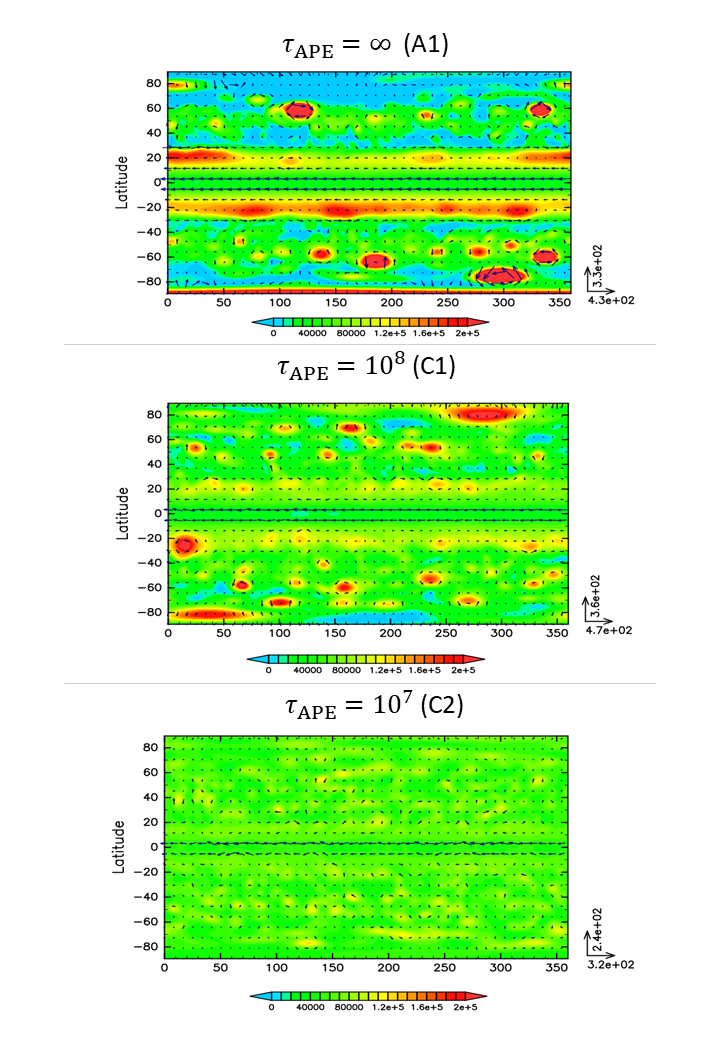
\includegraphics[clip,width=14cm]{./fig/result/case2/case2_phi.png}
    \caption{
      \footnotesize{ジオポテンシャルと速度ベクトル(3000 地球日).
上に$\tau_{\rm{APE}}$ の値とケース名を示す.
トーン値の範囲は$0:2 \times 10^5$である.
      }
    }
    \label{fig:case2_phi1}
  \end{center}
\end{figure}
%
%
\begin{figure}[ht]
  \begin{center}
    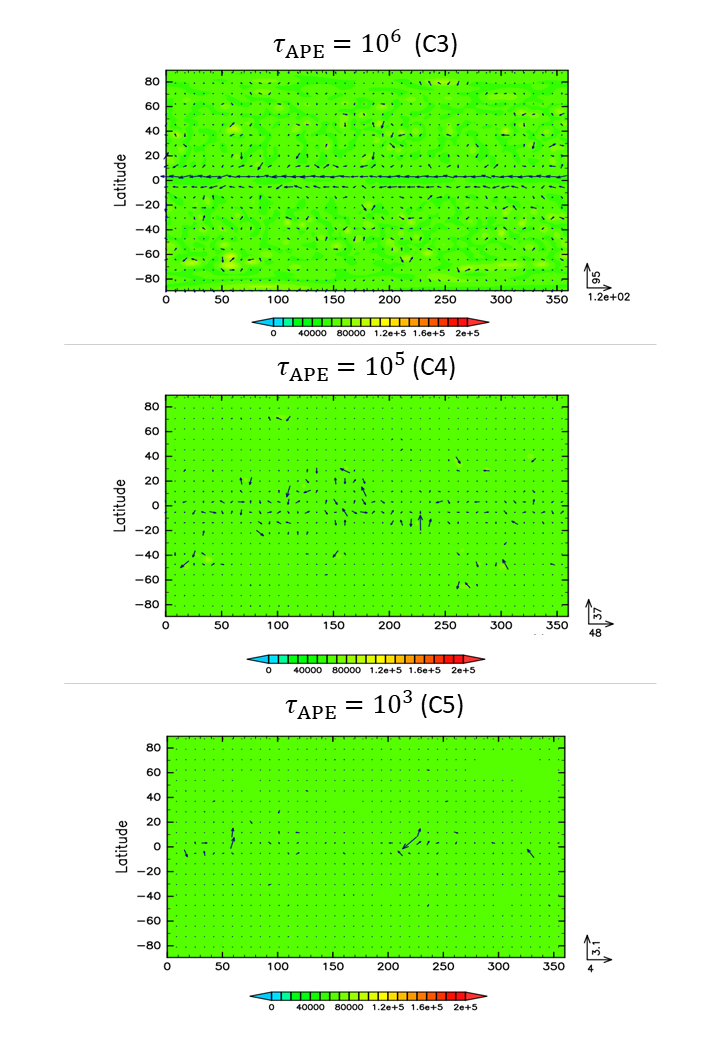
\includegraphics[clip,width=14cm]{./fig/result/case2/case2_phi2.png}
    \caption{
      \footnotesize{ジオポテンシャルと速度ベクトル(3000 地球日).
上に$\tau_{\rm{APE}}$ の値とケース名を示す.
トーン値の範囲は$0:2 \times 10^5$である.
      }
    }
    \label{fig:case2_phi2}
  \end{center}
\end{figure}
%
%
\begin{figure}[ht]
  \begin{center}
    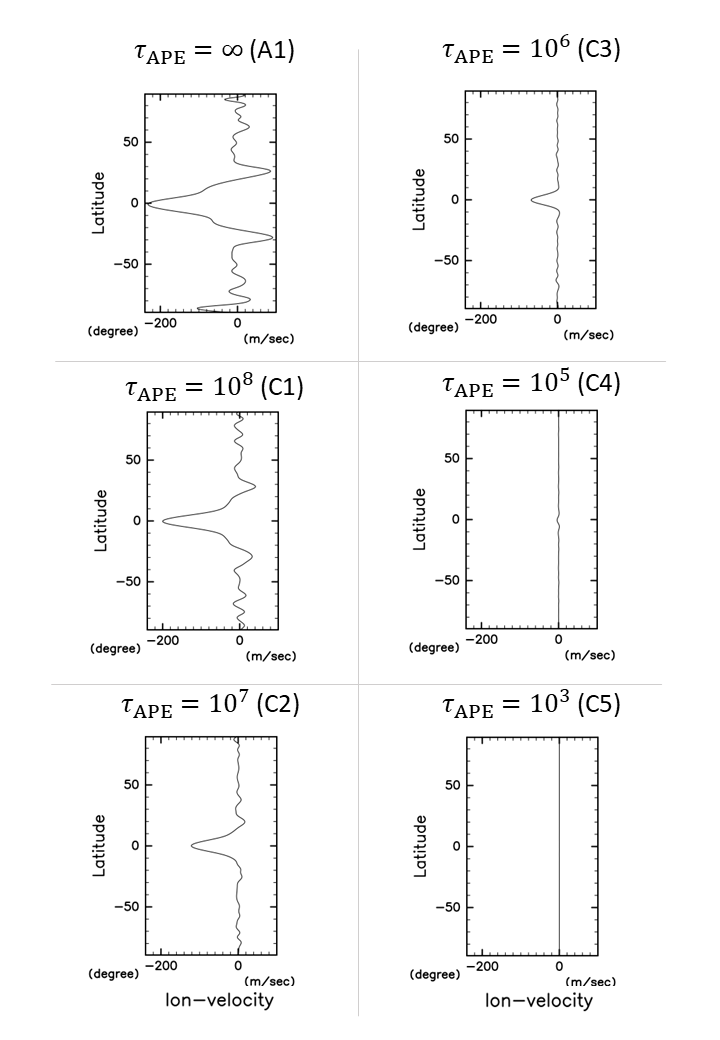
\includegraphics[clip,width=14cm]{./fig/result/case2/case2_vellon.png}
    \caption{
      \footnotesize{東西平均した東西風速(3000 地球日).
上に$\tau_{\rm{APE}}$ の値とケース名を示す.
      }
    }
    \label{fig:case2_vellon}
  \end{center}
\end{figure}
%
\begin{figure}[ht]
  \begin{center}
    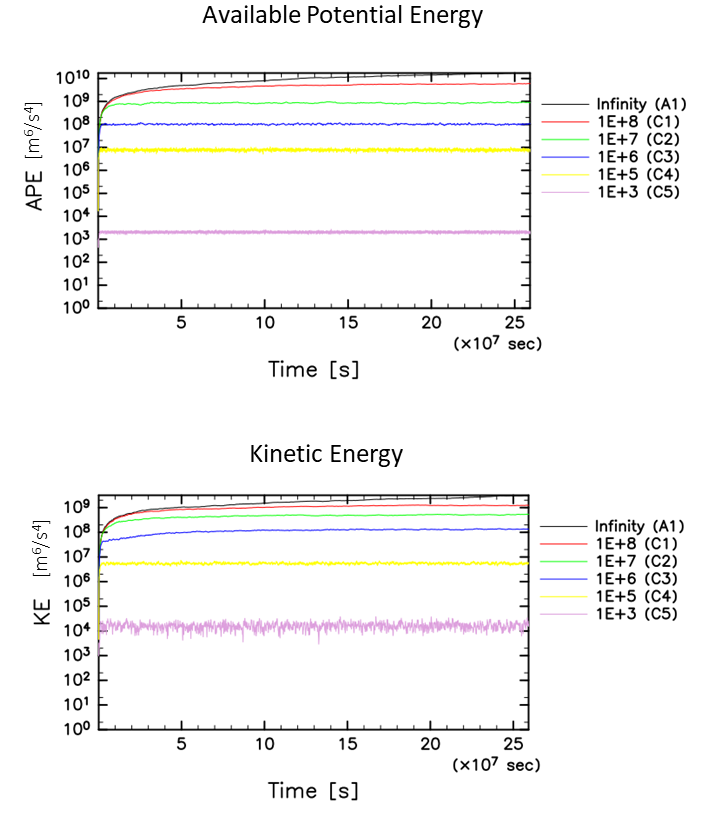
\includegraphics[clip,width=12cm]{./fig/result/case2/case2_apeke.png}
    \caption{
      \footnotesize{実験2の実験結果. 上 : 有効ポテンシャルエネルギー : APE ,
下 : 運動エネルギー : KE の時間発展.右上に$\tau_{\rm{APE}}$ の値と各線のケース名を示す.
      }
    }
    \label{fig:case2_apeke}
  \end{center}
\end{figure}

%%%%%%%%%%%%%%%%%% case3 : alpha %%%%%%%%%%%%%%%%%%%
\clearpage
\newpage
\section{実験3 : {$\alpha$} の変化による影響}
\label{sec:case3}
この節では質量強制の正負の割合である$\alpha$ の変化による影響を調べる.
$\alpha = 1.0 (~0.0)$ のとき正(負)の質量強制のみが与えられ,強制が与えられた位置で高気圧性(低気圧性)渦を形成する.
行ったケースは$\alpha = 1, 0.5, 0.0$ である.

結果(仮)
%%%%%%%%%%%%%%%%%%%%%%%%
\begin{itemize}
\item{$\alpha$ の値によって,極渦の空間スケール・レジームは変化しない.}
\item{$\alpha$ の値によって,東西風は変化しない.}
\end{itemize}
%

文章(仮) 

図\ref{fig:case3_nonqv},図\ref{fig:case3_vellon} に
それぞれのケースの無次元ポテンシャル渦度と東西平均した東西風速を示す.
このケースのBurger 数は$Bu = 4.64\times 10^{-4}$で\cite{Brueshaber2019}によれば
高気圧・低気圧性渦が共存する遷移レジームである.
%
図\ref{fig:case3_nonqv}を見てみると,確かにそのような特徴が見られ,
その特徴は$\alpha$の値によって,空間スケールやレジームが北極・南極域ともに変化しない.
%
また,図\ref{fig:case3_vellon}の東西平均した東西風速も
赤道域の東風ジェットの大きさ(約$-120 \rm{~m \cdot s^{-1}}$)や幅,
中緯度の西風ジェットが形成する緯度(約$\pm 30^\circ$)も目立った変化は見られない.
%
\begin{figure}[ht]
  \begin{center}
    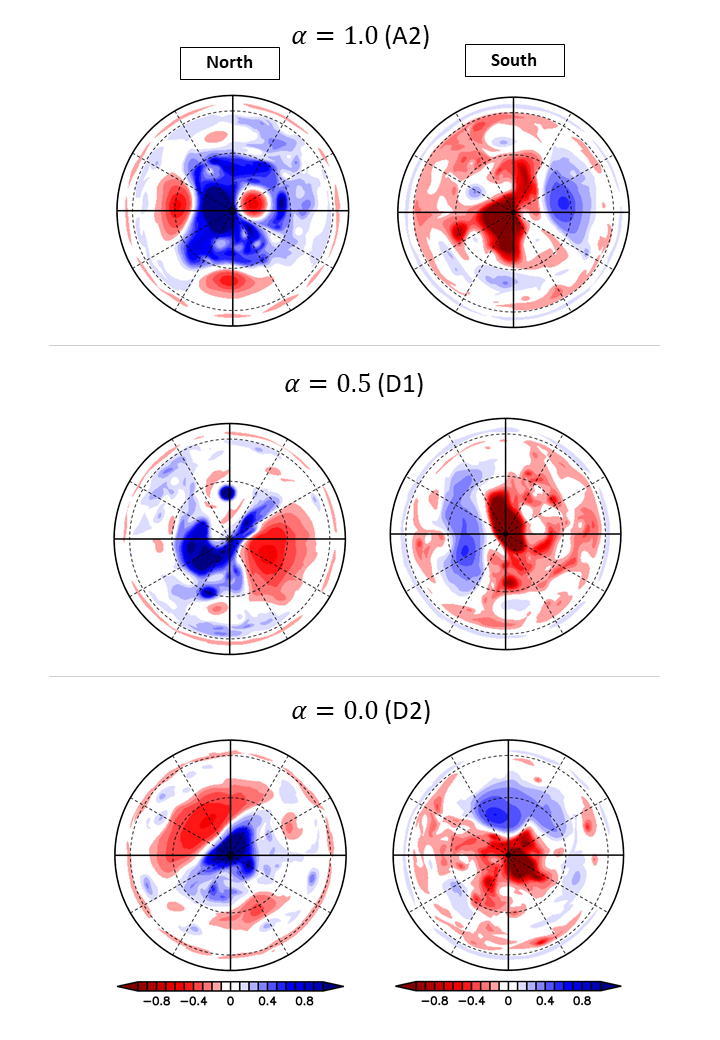
\includegraphics[clip,width=9cm]{./fig/result/case3/case3_nonqv.png}
    \caption{
      \footnotesize{無次元ポテンシャル渦度(3000 地球日).
左 : 緯度$90^\circ$ から見た球面投影.
右 : 緯度$-90^\circ$ から見た球面投影.
上に$\alpha$ の値とケース名を示す.
無次元ポテンシャル渦度のトーン値の範囲は$-1:1$である.
      }
    }
    \label{fig:case3_nonqv}
  \end{center}
\end{figure}
\clearpage
%
%
\begin{figure}[ht]
  \begin{center}
    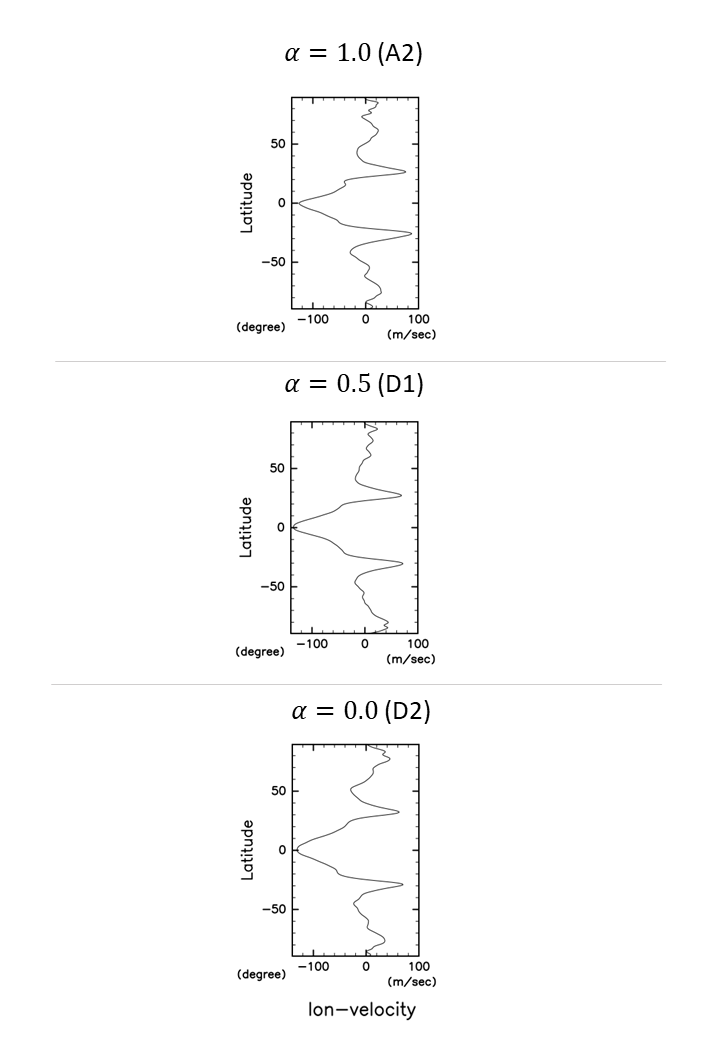
\includegraphics[clip,width=14cm]{./fig/result/case3/case3_vellon.png}
    \caption{
      \footnotesize{東西平均した東西風速(3000 地球日).
上に$\alpha$ の値とケース名を示す.
      }
    }
    \label{fig:case3_vellon}
  \end{center}
\end{figure}
%
%
%%%%%%%%%%%%%%%%%% case4 : R_storm %%%%%%%%%%%%%%%%%%%
\clearpage
\newpage
\section{実験4 : $R_{\rm{storm}}$ の変化による影響}
\label{sec:case4}
この節では質量強制の空間的大きさである$R_{\rm{storm}}$ の変化による影響を調べる.
\cite{Showman2007} によれば,$R_{\rm{storm}}$の中に
最低でも3個の格子点を含むとされている.
そのため,$R_{\rm{storm}}$を小さくすると
それに従い,解像度をあげなければならない.
行ったケースは${\rm{T341}} : R_{\rm{storm}} = 8.72 \times 10^5 ~(0.7^\circ), 
{\rm{T170}} : R_{\rm{storm}} = 2.62 \times 10^6 ~(2.1^\circ)$ であり,
それぞれのケースで$R_{\rm{storm}}$の中に約3個の格子点を含んでいる.
%

結果(仮)
%%%%%%%%%%%%%%%%%%%%%%%%
\begin{itemize}
\item{$R_{\rm{storm}}$ の値によって,極渦の空間スケール・レジームは変化しない.}
\item{$R_{\rm{storm}}$ の値によって,東西風速の大きさ中緯度の西風ジェットが形成する緯度が変化する.}
\end{itemize}
%

文章(仮) 

図\ref{fig:case4_nonqv}に無次元ポテンシャル渦度を示す.
このケースのBurger 数は$Bu = 4.64\times 10^{-4}$で\cite{Brueshaber2019}によれば
高気圧・低気圧性渦が共存する遷移レジームである.
%
$R_{\rm{storm}}$ の値をA1 に比べて,3分の1にしたE1 でも
遷移レジームの特徴が見られた.
%
東西平均した東西風速を見てみると
赤道域で東風ジェットが形成する.
また,$R_{\rm{storm}}$ を小さくしたことにより,注入されるエネルギーが減少,
結果として,赤道域の東風ジェットの風速が
A1 の約$200 \rm{m\cdot s^{-1}}$に比べ,
E1 では約$60 \rm{m \cdot s^{-1}}$となり,約3分の1小さくなる.
%
中緯度の西風ジェットが形成する緯度は,
A1 で約$\pm 30^\circ$, E1で約$\pm 20^\circ$ となる.
%
\begin{figure}[ht]
  \begin{center}
    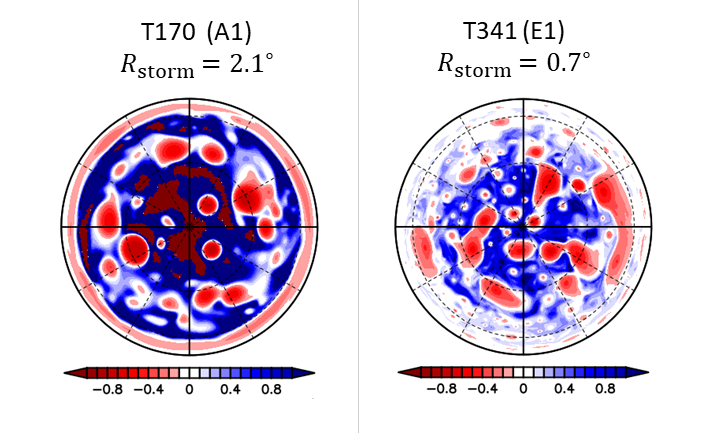
\includegraphics[clip,width=10cm]{./fig/result/case4/case4_nonqv.png}
    \caption{
      \footnotesize{緯度$90^\circ$ から見た球面投影の無次元ポテンシャル渦度(2000 地球日).
上に解像度と$R_{\rm{storm}}$ の値とケース名を示す.
無次元ポテンシャル渦度のトーン値の範囲は$-1:1$である.
      }
    }
    \label{fig:case4_nonqv}
  \end{center}
\end{figure}
%
%
\begin{figure}[ht]
  \begin{center}
    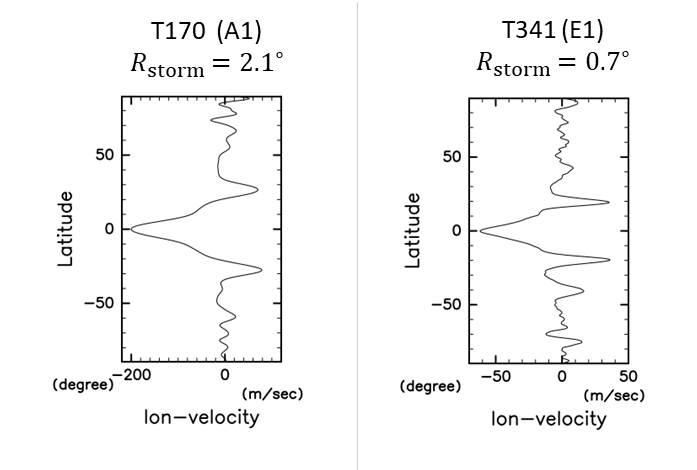
\includegraphics[clip,width=10cm]{./fig/result/case4/case4_vellon.png}
    \caption{
      \footnotesize{東西平均した東西風速(2000 地球日).
上に解像度と$R_{\rm{storm}}$ の値とケース名を示す.
      }
    }
    \label{fig:case4_vellon}
  \end{center}
\end{figure}
%

%
%
\def\chap4{議論とまとめ}
\chapter{\chap4}
\label{chap:4}
\markright{4 \chap4}
%
以下では,\ref{chap:3}章での実験結果で得られた
Burger 数が大きい場合で得られる低気圧性極渦と
緩和が大きくない場合,全てのケースで見られた赤道域の東風ジェットと
中緯度域の西風ジェットの形成について議論を行う.
\section{極域への低気圧性渦度の集積}
\label{sec:considpolar}
\ref{sec:case1} 節の実験では質量強制の正負の割合$\alpha$ は$1.0$ のため,
図\ref{fig:consid_nonqv_a3} の5日目の計算結果を見て分かるように
層の厚さを局所的に増やし,高気圧性渦を作り出す.
50日目になると,低気圧性渦が形成し始め,
3000 日になると,極を中心に強力な低気圧性渦が出来る.
%
低気圧性の渦度が極域に集まる理由として
ベータドリフトが考えられている.
%
ベータドリフトとは惑星渦度の緯度方向勾配による
ベータ効果により,渦が自身のまわりに
2次的な渦を作り出し,その渦の効果で移動するというものである.
これは,次のように理解することができる.
強制散逸のない球面浅水系では
ポテンシャル渦度 : $q$ が保存する.
\begin{align}
q = \frac{\zeta + f}{h}. \label{qv}
\end{align}
ここで,図\ref{fig:betadrift}のように
北半球のある緯度に低気圧性渦が置かれている状況を考える.
この渦の上下にある流体がこの低気圧性渦の影響を受け,
移動したとする.
低緯度側に移動してきた流体は$f$が小さくなるが
式(\ref{qv})は保存しなければならないため,$\zeta$ が増えなければいけない.
高緯度側に移動した流体も同様の効果を受け,渦度を持つ.
その結果,その2次的な渦の影響を受け,
元々の低気圧性渦が高緯度へ移動する.
初期に高気圧性渦が位置していた場合,同様に考えると低緯度側へ移動する.
その結果,極での低気圧性渦度の累積が起きると考えられる.
\begin{figure}[ht]
  \begin{center}
    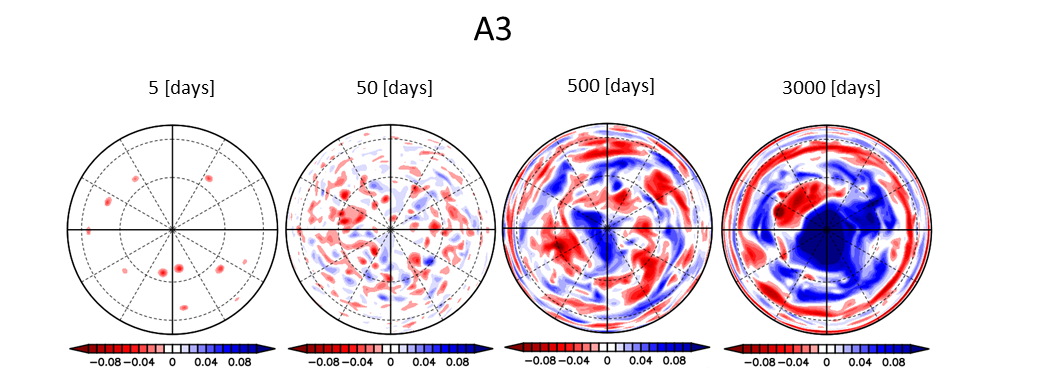
\includegraphics[clip,width=14cm]{./fig/consideration/nonqv_a3.png}
    \caption{
      \footnotesize{緯度$90^\circ$ から見た球面投影の無次元ポテンシャル渦度.
上にケース名を示す.
左から5, 50, 500, 3000 日の計算結果.
無次元ポテンシャル渦度のトーン値の範囲は$-0.1:0.1$である.
      }
    }
    \label{fig:consid_nonqv_a3}
  \end{center}
\end{figure}
%
\begin{figure}[ht]
  \begin{center}
    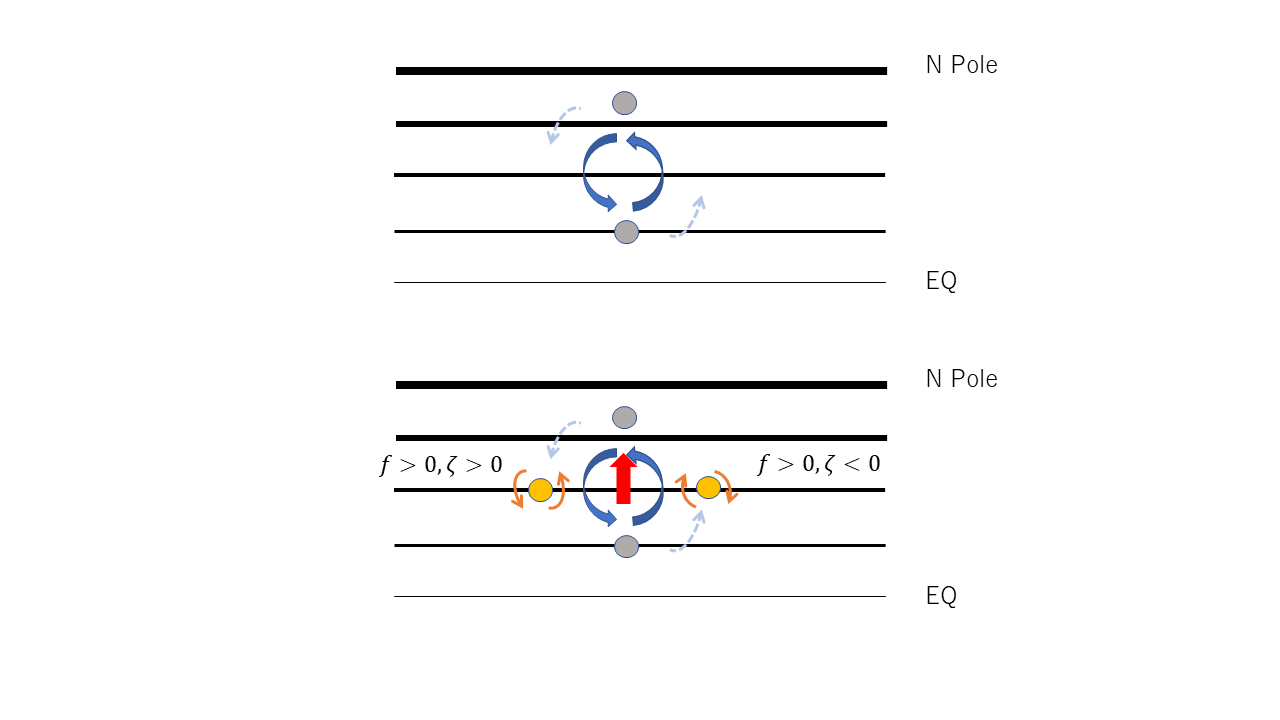
\includegraphics[clip,width=14cm]{./fig/consideration/betadrift_1.png}
    \caption{
      \footnotesize{ベータドリフトの模式図.
上 : 初期に位置している低気圧性渦.
下 : 低気圧性渦のまわりの流体が移動し,2次的な渦を形成.
低気圧性渦自体を高緯度へ移流させる.
      }
    }
    \label{fig:betadrift}
  \end{center}
\end{figure}
\clearpage
%
\newpage
%
巨大惑星で観測される極渦やジェットといった構造が
雷雲による強制によるものかを調べるために
雷雲を想定した質量強制を加えた,1.5層浅水球面実験を全球で行った.
%
その結果,
Burger 数の値によって,極渦のレジームが変化した(実験1).
%
Burger 数が比較的小さい$Bu = 9.72 \times 10^{-5}$の場合, 複数の高気圧性渦が形成する.
Burger 数$Bu = 1.46 \times 10^{-3}$ の場合, 高気圧性渦と低気圧性渦が混在するレジームが見られた.
Burger 数が大きい$Bu = 1.46 \times 10^{-3}$の場合,土星で見られるような単一低気圧性渦が支配的になることがわかった.
Burger 数を変形半径と惑星半径,それぞれを変化させたが,大きな違いは見られなかった.
質量強制の正負の割合$\alpha $ (実験3) や空間的大きさ$R_{\rm{storm}}$ (実験4) を変化させ,
その影響を調べたが大きな影響は見られなかった.
この計算結果はBurger 数が極域のレジームに重要だと
主張した \cite{Brueshaber2019} の結果と整合的である.
%
東西風分布は$Bu \leq 1.46 \times 10^{-3}$ で
で赤道域の東風ジェットと中緯度約$\pm 20^\circ \sim 30^\circ$ で西風ジェットが形成した.
Burger 数の値が大きくなると,赤道域のジェットは見られなくなり,
低気圧性極渦による西風が大きくなることがわかった.
%
\cite{Showman2007} と同様のパラメータを用いたA3 のケースで
赤道域のジェットの風速を比較してすると我々の計算が約10倍大きくなることがわかった.
これは,\cite{Showman2007} の計算結果が領域計算により,
計算領域外からの運動量輸送の影響を示唆している.

局所的な緩和の時間スケールである$\tau_{\rm{APE}}$ の値によって,
渦の空間スケールや東西風速の大きさが変化することがわかった.
$\tau_{\rm{APE}} = \infty $ のケースでは,質量強制により,
エネルギーが継続的に増加し,空間スケールの大きな渦や風速の大きな
赤道域の東風ジェットを形成する.
$\tau_{\rm{APE}}$が有限の場合,エネルギーが逆カスケードするまえに
散逸し,空間スケールが小さくなることがわかった.
また,ある時間でエネルギーの注入率と除去率がつり合い,
APE とKE が平衡することがわかった.
これは今回の積分時間の妥当性を示す.

以上の結果から雷雲による強制により,
巨大惑星で見られる単一の低気圧性渦は形成したが,木星で見られる
複数の低気圧性渦の規則的は配置はみられなかった.
また,風速分布はジェットが形成する全てのケースで
赤道域で東風,また中緯度で西風ジェットが形成した.
木星,土星でみられる赤道域の西風ジェットは見られなかった.

今後は今回の計算結果の詳細な解析と
考慮しなかったら質量強制の分布など
他のパラメータ依存性を調べる必要がある.

%%% Appendix %%%
%%%%%%%%%%%%%%%%
%\setcounter{chapter}{1} % chapter の番号をゼロにリセットする
%\setcounter{section}{0} % section の番号をゼロにリセットする
\stepcounter{chapcounter}
\stepcounter{seccounter}

\renewcommand{\thesection}{\Alph{section}} % 数字ではなくアルファベットで数える

\def\thesection{\Alph{section}}
\def\theequation{\Alph{section}.\arabic{equation}}

\chapter*{付録}
\addcontentsline{toc}{chapter}{付録}
%%  A  %%
\def\apetitleA{: 1.5層浅水方程式系の導出}
\def\apeA{\Alph{section} \apetitleA}
\section{\apetitleA}
\label{ape:A}
\markright{\apeA}
%% Appendix A %%
%%%%%%%%%%%%%%%%
\setcounter{subsection}{0}
\setcounter{subsubsection}{0}
\setcounter{figure}{0}
\setcounter{table}{0}
\setcounter{equation}{0}
\renewcommand{\thesubsection}{\Alph{section}.\arabic{subsection}} 
\renewcommand{\thesubsubsection}{\Alph{section}.\arabic{subsection}.\arabic{subsubsection}} 
\renewcommand{\thefigure}{\Alph{section}.\arabic{figure}}
\renewcommand{\thetable}{\Alph{section}.\arabic{table}}
%
$B$3$3$G$O!$(B\cite{Vallis2017} 3.2$B@a(B $BM-8z=ENO$NJ}Dx<07O$r;29M$K!$(B
1.5$BAX@u?e%b%G%k$NJ}Dx<0$rF3=P$9$k!%(B
\subsection*{$B!&(B1.5 $BAX@u?e%b%G%k$N35MW(B}
$B@u?e7O$G:G$bC1=c$J(B1$BAX%b%G%k$O(B
$BL)EY$,JQ2=$7$J$$0lAX$NN.BNAX$r9M$($F$$$k!%(B
%
%
\begin{figure}[b]
 \begin{center}
 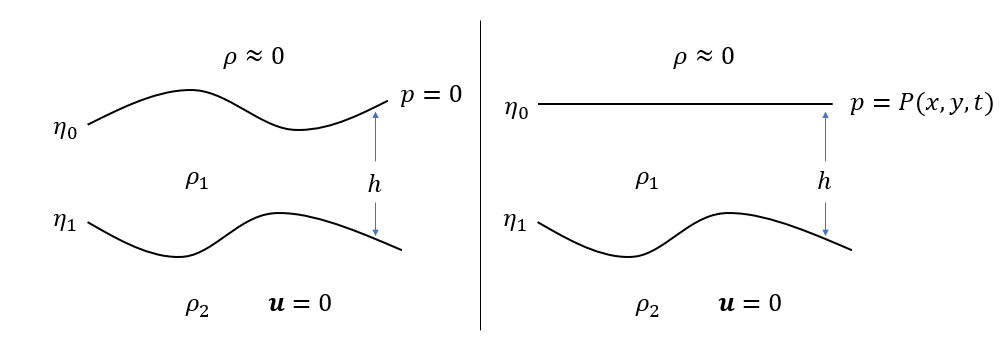
\includegraphics[clip,width=13cm]{./appendix/A/fig/one-half-fig1.png}
 \end{center}
 \caption{1.5$BAX@u?eJ}Dx<07O$NLO<0?^!!(B(\cite{Vallis2017} $B$N?^(B3.3 $B$r2~JQ(B).
$B:8$O<+M3I=LL6a;w!$1&$O9dBNI=LL6a;w$G$"$k!%(B
$B>eAX$N8|$5(B$h$$B$O>eAX$N9b$5(B$\eta_0$$B$H2<AX$N9b$5(B$\eta_1$$B$rMQ$$$F!$(B
$h=\eta_0 - \eta_1$$B$G=q$+$l$k!%(B
} 
 \label{figA1}
\end{figure}
%
$B$7$+$7!$8=<B$NN.BN$NL)EY$OJQ2=$9$k$O$:$G$"$k!%(B
$BFC$K@.AX$7$F$$$l$P!$1tD>J}8~$KJQ2=$9$k$H9M$($i$l$k!%(B
1.5$BAX%b%G%k$G$O>eAX$O3hF0E*!$(B
$B2<AX$OL58B$K?<$/@E;_$7$?L)EY$N0[$J$k(B2$B$D$NN.BNAX$r9M$(!$(B
$BC1=c$G$O$"$k$,1tD>J}8~$NL)EYJQ2=$r9MN8$9$k!%(B
%
$B3$MN$G$O2<AX$O$[$H$s$I@E;_$7!$(B
$B1?F0$N$"$k>eAX$O?t(B100 m $B$N8|$5$G$"$k$?$a!$(B
$B$3$N%b%G%k$,;H$o$l$k$3$H$,$"$k!%(B
%
$B?^(B\ref{figA1}$B$K(B1.5$BAX%b%G%k$NLO<0?^$r<($9!%(B
$B$3$3$G!$(B$\eta_0$$B$O>eAX$N9b$5!$(B
$\eta_1$$B$O2<AX$N9b$5!$(B$h$$B$O>eAX$N8|$5!$(B
$B>eAX!$2<AX$NL)EY$O$=$l$>$l(B$\rho_1, \rho_2~(\rho_1 < \rho_2)$ $B$G$"$k!%(B
$B>eC<$N6-3&>r7o$O<+M3I=LL$H9dBNI=LL$N(B2$B$D$N>l9g$,$"$k!%(B
\cite{Showman2007}, \cite{Brueshaber2019} $B$G$O(B
$B9dBNI=LL6a;w$rMQ$$$F$$$k$H9M$($i$l$k!%(B
$B0J2<$G$O$=$l$>$l$N6-3&>r7o$N>l9g$GJ}Dx<07O$rF3$/!%(B
%
%\cite{Showman2007} $B$G$O(B
%$B>eAX$O@ENO3XE*$K0BDj$7$?BPN.7w>eIt(B (5 - 10 bar $B$N(B
%$B?e$N6E7k%l%Y%kIU6a$+$i>e$NAX$N8|$5(B)$B!$(B
%$B2<AX$OL58B$K?<$/CfN)E*$K@.AX2=$7$?AX$r(B
%$B9M$($k$H5-:\$7$F$$$k!%(B
%
\subsection*{$B!&<+M3I=LL6a;w(B}
\subsubsection*{$B1?F0NLJ}Dx<0(B}
$B$^$:$O>eAX$K$D$$$F9M$($k!%>eAX$N@E?e05$N<0$O(B
\begin{equation}
\frac{\partial p_1}{\partial z}=-\rho_1 g. \label{eq:A1}
\end{equation}
$B$3$l$r!$>eAX$N>eC<(B$\eta_0$ $B$+$i$"$k?<$5(B$z$ $B$^$G@QJ,$9$k$H(B
\begin{equation}
\int_0^{p_1} dp= -\rho_1 g  \int_{\eta_0}^z dz. \label{eq:A2}
\end{equation}
$B<+M3I=LL6a;w$G$O>eAX$N>eC<$G(B$p(\eta_0) = 0$$B$J$N$G!$(B
\begin{equation}
p_1 (x, y, z, t) = \rho_1 g  (\eta_0 - z). \label{eq:A3}
\end{equation}
$B<0(B(\ref{eq:A3})$B$N?eJ?8{G[$r$H$k$H!$(B
\begin{align}
\nabla_z p_1 &= \rho_1 g \nabla_z \eta_0, \notag \\
\frac{1}{\rho_1} \nabla_z p_1 &=  g \nabla_z \eta_0. \label{eq:A4}
\end{align}
$B$3$3$G!$(B
\begin{align}
\nabla_z&=\left(\frac{\partial}{\partial x},\frac{\partial}{\partial y}\right). \notag
\end{align}
%

$B<!$K2<AX$K$D$$$F9M$($k!%(B
$B2<AX$N@E?e05$N<0$O(B
\begin{equation}
\frac{\partial p_2}{\partial z}=-\rho_2 g. \label{eq:A5}
\end{equation}
$B$3$l$r!$2<AX$N>eC<(B$\eta_1$ $B$+$i$"$k?<$5(B$z$ $B$^$G@QJ,$9$k$H(B
\begin{align}
\int_{p_1}^{p_2} dp= -\rho_2 g  \int_{\eta_1}^z dz, \notag \\
p_2 - p_1 = \rho_2 g  (\eta_1 -  z). \label{eq:A6}
\end{align}
$p_1$ $B$O<0(B(\ref{eq:A3})$B$G(B $z=\eta_1$$B$H$7$?CM$J$N$G(B
\begin{align}
p_2  &= p_1  + \rho_2 g  (\eta_1  - z) \notag \\
     &= \rho_1 g (\eta_0 - \eta_1) + \rho_2 g  (\eta_1  - z) \notag \\
     &= \rho_1 g (\eta_0 - \eta_1) + \rho_2 g  (\eta_1  - z).  \label{eq:A7}
\end{align}
%
$B<0(B(\ref{eq:A7})$B$N?eJ?8{G[$r$H$k$H!$(B
\begin{align}
\nabla_z p_2 &= \rho_1 g  (\nabla_z \eta_0 - \nabla_z \eta_1) + \rho_2 g  \nabla_z \eta_1   \notag \\
& = \rho_1 g \nabla_z \eta_0 +  \rho_1 g \frac{(\rho_2 - \rho_1)}{ \rho_1 }  \nabla_z \eta_1 \notag \\
& = \rho_1 g \nabla_z \eta_0 +  \rho_1 g'  \nabla_z \eta_1. \label{eq:A8} 
\end{align}
$B$3$3$G!$(B$g'$ $B$ODc8:=ENO2CB.EY(B(reduced gravity) 
\begin{align}
g' = g \frac{(\rho_2 -\rho_1)}{\rho_1}  \notag 
\end{align}
$B$G$"$k!%2<AX$O1?F0$,$J$$$N$G!$<0(B(\ref{eq:A8}) $B$N(B
$B:8JU$N05NO8{G[(B$\nabla_z p_2 $$B$O(B 0$B$K$J$k!%(B
$B$h$C$F!$(B
\begin{align}
 g \nabla_z \eta_0 = -  g'  \nabla_z \eta_1 . \label{eq:A9}
\end{align}
$B<0(B(\ref{eq:A4}) $B$h$j(B
\begin{align}
 \frac{1}{\rho_1} \nabla_z p_1  = -  g'  \nabla_z \eta_1 . \label{eq:A10}
\end{align}
%
$B>eAX$N2sE>$N8z2L$r4^$`HsG4@-N.BN$N1?F0NLJ}Dx<0$O(B
\begin{equation}
%\DP{\Dvect{u_1}}{t}+(\Dvect{u_1} \cdot \nabla)\Dvect{u_1}=
%-f\Dvect{k}\times \Dvect{u_1}-\frac{1}{\rho_1}\nabla_z p_1. \label{eq:A11}
\DD{\Dvect{u_1}}{t} + \frac{1}{\rho_1}\nabla_z p_1 + f\Dvect{k}\times \Dvect{u_1} = 0. \label{eq:A11}
\end{equation}
$B$3$3$G!$(B$\Dvect{k}$$B$O(B$z$$BJ}8~$NC10L%Y%/%H%k$G$"$k!%(B
$B<0(B(\ref{eq:A11})$B$K<0(B(\ref{eq:A10})$B$rBeF~$9$k$H(B
\begin{equation}
\DD{\Dvect{u_1}}{t}  - g' \nabla_z\eta_1 + f\Dvect{k}\times \Dvect{u_1} = 0 \label{eq:A12}
\end{equation}
$B$H$J$k!%(B
%
\subsubsection*{$BO"B3$N<0(B}
$BO"B3$N<0$O(B1$BAX$N@u?e7O$HF1MM$K9M$($k$3$H$,$G$-!$(B
\begin{equation}
\DP{g'h}{t}+\nabla_z (g'h\Dvect{u_1})=0$B!%(B\label{eq:A13}
\end{equation}
$B$^$H$a$k$H(B
\begin{itembox}[l]{$B<+M3I=LL6a;w(B}
\begin{align}
&\text{$B!&1?F0NLJ}Dx<0(B}$B!!(B\quad \DD{\Dvect{u_1}}{t}  - g'\nabla_z\eta_1 + f\Dvect{k}\times \Dvect{u_1} = 0
$B!!(B\tag{A.11} \\
&\text{$B!&O"B3$N<0(B}$B!!(B\qquad \DP{g'h}{t}+\nabla_z (g'h\Dvect{u_1})=0 \tag{A.12}$B!%(B
\end{align}
\end{itembox}
%
\subsection*{$B!&9dBNI=LL6a;w(B}
$BI=LL$G$N1?F0$,>.$5$$$J$i$P!$9dBNI=LL$rCV$$$?$H$$$&6a;w$r$7$F$b$h$$$@$m$&!%(B
$B>eC<$K$U$?$r$9$k$3$H$G!$>eC<$N>e2<1?F0$O5v$5$l$J$/$J$k!%(B
$B$=$N05NO$N6/@)$r(B$P(x, y, t)$$B$H$9$k!%(B
$B$^$?!$>eAX$N>eC<$r4p=`LL$K$H$j!$$=$3$G(B$z=0$$B$H$9$k(B ($\eta_0 = 0$)$B!%(B
$B<+M3I=LL6a;w$HF1MM$K>eAX$G$N@E?e05$N<0$r(B$z=0$$B$+$i$"$k?<$5(B$z$$B$^$G@QJ,$9$k$H(B
\begin{align}
\int_P^{p_1} dp= -\rho_1 g  \int_{0}^z dz, \notag \\
p_1 - P   = - \rho_1 g z. \label{eq:A14}
\end{align}
$B<0(B(\ref{eq:A14})$B$N?eJ?8{G[$r$H$k$H!$(B
\begin{align}
\nabla_z p_1 &= \nabla_z P. \label{eq:A15}
\end{align}
$B2<AX$N@E?e05$N<0$r(B$\eta_1$$B$+$i$"$k?<$5(B$z$$B$^$G@QJ,$9$k$H(B
\begin{align}
\int_{p_1}^{p_2} dp &= -\rho_2 g  \int_{\eta_1}^z dz, \notag \\
p_2 - p_1 &= \rho_2 g (\eta_1 - z), \notag \\
p_2 &= p_1 + \rho_2 g (\eta_1 - z). \label{eq:A16}
\end{align}
$p_1$ $B$K<0(B(\ref{eq:A14})$B$G(B$ z=\eta_1$ $B$K$7$?$b$N$rBeF~$9$l$P(B
\begin{align}
p_2 & = -\rho_1 g \eta_1 + \rho_2 g (\eta_1 - z) + P$B!!(B\notag \\
& = \rho_1 g h - \rho_2 g (h - z) + P. \label{eq:A17}
\end{align}
$B?eJ?8{G[$r$H$k$H(B
\begin{align}
\nabla_z p_2 & = - g (\rho_2 - \rho_1) \nabla_z h  + \nabla_z P, \notag \\
& = - \rho_1 g' \nabla_z h  + \nabla_z P . \label{eq:A18}
\end{align}
$B2<AX$G$O1?F0$,$J$$$N$G(B$\nabla_z p_2 = 0$$B!%$h$C$F(B
\begin{align}
\frac{1}{\rho_1 } \nabla_z P =   g' \nabla_z h. \label{eq:A19}
\end{align}
$B<0(B(\ref{eq:A15})$B$h$j(B
\begin{align}
\frac{1}{\rho_1} \nabla_z p_1 =  g' \nabla_z h. \label{eq:A20}
\end{align}
$B<0(B(\ref{eq:A11})$B$K<0(B(\ref{eq:A20})$B$rBeF~$9$k$H(B
\begin{equation}
\DD{\Dvect{u_1}}{t} + g' \nabla_z h + f\Dvect{k}\times \Dvect{u_1} = 0 \label{eq:A21}
\end{equation}
$B$H$J$k!%(B
%
$B$^$H$a$k$H(B
\begin{itembox}[l]{$B9dBNI=LL6a;w(B}
\begin{align}
&\text{$B!&1?F0NLJ}Dx<0(B}$B!!(B\quad \DD{\Dvect{u_1}}{t} + g'\nabla_z h
 + f\Dvect{k}\times \Dvect{u_1}  =0
$B!!(B\tag{A.21}\\
&\text{$B!&O"B3$N<0(B}$B!!(B\qquad \DP{g'h}{t}+\nabla_z (g'h\Dvect{u_1})=0 \tag{A.12}$B!%(B
\end{align}
\end{itembox}
%
$B9dBNI=LL6a;w$NJ}Dx<07O$O(B
1$BAX%b%G%k$NDlLLCO7A$,$J$$>l9g$N(B
$BJ}Dx<07O$N=ENO2CB.EY(B : $g$ $B$,Dc8:=ENO2CB.EY(B : $g'$ $B$KCV$-$+$o$k$@$1$G$"$k!%(B
%
$BK\8&5f$O$3$N9dBNI=LL6a;w$rMQ$$$k!%(B

%
\newpage
%
%%  B  %%
\def\apetitleB{: モデルで使用した方程式系}
\def\apeB{\Alph{section} \apetitleB}
\section{\apetitleB}
\label{ape:B}
\markright{\apeB}
%% Appendix B %%
%%%%%%%%%%%%%%%%
\setcounter{subsection}{0}
\setcounter{subsubsection}{0}
\setcounter{figure}{0}
\setcounter{table}{0}
\setcounter{equation}{0}
\renewcommand{\thesubsection}{\Alph{section}.\arabic{subsection}} 
\renewcommand{\thesubsubsection}{\Alph{section}.\arabic{subsection}.\arabic{subsubsection}} 
\renewcommand{\thefigure}{\Alph{section}.\arabic{figure}}
\renewcommand{\thetable}{\Alph{section}.\arabic{table}}
%
$B$3$3$G$O<B:]$K%b%G%kFb$G7W;;$7$?J}Dx<07O$r<($9!%(B
\subsection*{$B!&12EY!&H/;67?$N1?F0NLJ}Dx<0$X$NJQ7A(B}
$B1?F0NLJ}Dx<0(B(\ref{eq:eq1}) $B$O%*%$%i!<7A<0$G=q$/$H(B
\begin{align}
\DP{\Dvect{u}}{t} + (\Dvect{u}\cdot \nabla)\Dvect{u} +  g' \Dgrad h + f \Dvect{k} \times \Dvect{u} = -\Dvect{D}_{\Dvect{u}},  \label{ape:B1}
\end{align}
$B$3$3$G!$:8JUBh(B2$B9`$N0\N.9`$NItJ,$rJQ7A$9$k$H(B
\begin{align}
(\Dvect{u}\cdot \nabla)\Dvect{u} = \nabla \left ( \frac{\Dvect{u}\cdot \Dvect{u}}{2} \right) +\zeta \Dvect{k}\times \Dvect{u} \label{ape:B2}
\end{align}
$B$H$J$k!%$3$l$r<0(B(\ref{ape:B1})$B$KBeF~$9$k$H(B
\begin{align}
& \DP{\Dvect{u}}{t} +  \nabla \left ( \frac{\Dvect{u}\cdot \Dvect{u}}{2} \right) +\zeta \Dvect{k}\times \Dvect{u} +  g' \Dgrad h + f \Dvect{k} \times \Dvect{u} = -\Dvect{D}_{\Dvect{u}},  \notag \\
& \DP{\Dvect{u}}{t} +  \nabla \left ( \frac{\Dvect{u}\cdot \Dvect{u}}{2}  +  g' \Dgrad h \right) +
 (\zeta + f ) \Dvect{k}\times \Dvect{u}   = -\Dvect{D}_{\Dvect{u}} \label{ape:B3}
\end{align}
$B$H$J$k!%(B
$B<0(B(\ref{ape:B3})$B$N2sE>$HH/;6$r$H$k$H!$$=$l$>$l(B
\begin{align}
\DP{\zeta}{t}&=-\Ddiv (\zeta+f)\Dvect{u} - D_\zeta ,\label{ape:B4} \\
\DP{D}{t}&=\Dvect{k}\cdot \Drot (\zeta+f)\Dvect{u} 
-\nabla^2 \left(g' h  +\frac{\Dvect{u}\cdot \Dvect{u}}{2}\right) -D_D. \label{ape:B5}
\end{align}
$B$G$"$k(B\footnote{
$B<0(B(\ref{ape:B5})$B$N:8JUBh(B3$B9`$K2sE>1i;;;R$r:nMQ$5$;$k$H(B
\begin{align}
-{\rm{\hat{\bf k}}}\cdot \Drot \left [ (\zeta+f){\rm{\hat{\bf k}}}\times \Dvect{v} \right ]&=-{\rm{\hat{\bf k}}}\cdot \Drot \left [ (\zeta+f) 
\left (
\begin{array}{c}
0 \\
0 \\
1
\end{array} \right )
\times 
\left (
\begin{array}{c}
u \\
v \\
w
\end{array} \right )
\right ] \notag \\
&=-{\rm{\hat{\bf k}}}\cdot \Drot \left [ (\zeta+f) 
\left ( 
\begin{array}{c}
-v \\
u \\
0
\end{array} \right) 
\right ] \notag \\
&=-{\rm{\hat{\bf k}}}\cdot  \left [ (\zeta+f) 
\left ( 
\begin{array}{c}
-\DP{u}{z} \\
-\DP{v}{z} \\
\DP{u}{x}+\DP{v}{y}
\end{array} \right) 
\right ] \notag \\
&= -\Ddiv (\zeta+f) \Dvect{v}. \notag
\end{align}

$B$^$?!$H/;61i;;;R$r:nMQ$5$;$k$H(B
\begin{align}
- \Ddiv \left [ (\zeta+f){\rm{\hat{\bf k}}}\times \Dvect{v} \right ] 
&={\rm{\hat{\bf k}}} \cdot \Drot (\zeta+f)\Dvect{v}.\notag
\end{align}$B$3$3$G!$%Y%/%H%k8x<0(B$\Ddiv (\Dvect{A}\times \Dvect{B})=\Dvect{B}\cdot (\Drot \Dvect{A})-\Dvect{A}\cdot \Drot \Dvect{B}$$B$rMQ$$$?!%(B
}$B!%(B
$B5eLL:BI87O$G$NJ*<AHyJ,!$H/;6!$8{G[!$2sE>$O(B
\begin{align}
\frac{D\phi}{Dt}&=\DP{\phi}{t}+\frac{u}{a\cos{\vartheta}}\DP{\phi}{\lambda}
+\frac{v}{a}\DP{\phi}{\vartheta}, \label{ape:B6} \\
\Ddiv \Dvect{A}&=\frac{1}{a\cos{\vartheta}}\left[\DP{A_\lambda}{\lambda}
+\DP{(A_\vartheta \cos{\vartheta})}{\vartheta}\right ], \label{ape:B7} \\
\nabla \phi&=\frac{\Dvect{i}}{a\cos{\vartheta}}\DP{\phi}{\lambda}
+\frac{\Dvect{j}}{a}\DP{\phi}{\vartheta},  \label{ape:B8} \\ 
\Drot \Dvect{A}&=\frac{1}{r^2\cos{\vartheta}}
\begin{vmatrix}
\Dvect{i}r\cos{\vartheta} & \Dvect{j}r & \Dvect{k} \\
\DP{}{\lambda} & \DP{}{\vartheta} & \DP{}{r} \\
A_\lambda r \cos{\vartheta} & A_\vartheta r &A_r \label{ape:B9}
\end{vmatrix}$B!%(B
\end{align}
$B$3$l$rMQ$$$F!$<0(B(\ref{ape:B4}), (\ref{ape:B5})$B$r=q$-2<$;$P(B
\begin{align}
\DP{\zeta}{t}&=-\frac{1}{a\cos{\vartheta}}\DP{}{\lambda}
[(\zeta+f)u]-\frac{1}{a\cos{\vartheta}}\DP{}{\vartheta}[(\zeta+f)v\cos{\vartheta}] - D_\zeta , \label{ape:B10} \\
\DP{D}{t}&=\frac{1}{a\cos{\vartheta}}\DP{}{\lambda}  
[(\zeta+f)v]-\frac{1}{a\cos{\vartheta}}\DP{}{\vartheta}[(\zeta+f)u\cos{\vartheta}] \notag \\
&-\nabla^2 \left [ g' h + E \right ] -D_D. \label{ape:B11}
\end{align}
$B$3$3$G!$(B$E$$B$O1?F0%(%M%k%.!<$G(B$E=(u^2 + v^2)/2$$B!%(B
$\nabla^2$$B$O(B
\begin{align}
\nabla^2=\frac{1}{a^2 \cos{\vartheta}^2}\DP[2]{}{\lambda}
+\frac{1}{a^2\cos{\vartheta}}\DP{}{\vartheta} \left (
\cos{\vartheta} \DP{}{\vartheta}\right ). \label{ape:B12}
\end{align}
%
\subsection*{$B!&%5%$%s0^EY$X$NJQ7A(B}
$U=u\cos \vartheta, V=v\cos \vartheta$$B$H(B$\mu = \sin \vartheta$$B$rMQ$$!$(B
$B%5%$%s0^EY$K=q$-$+$($k$H(B
%
\begin{align}
\DP{\zeta}{t} &= - \frac{1}{a (1-\mu^2)}
\DP{}{\lambda} [(\zeta + f)U] 
- \frac{1}{a}
\DP{}{\mu} [(\zeta + f)V] - D_\zeta, \label{ape:B13} \\
%
\DP{D}{t} &=  \frac{1}{a(1-\mu^2)}
\DP{}{\lambda} [(\zeta + f)V] 
- \frac{1}{a}
\DP{}{\mu} [(\zeta + f)U] \notag \\
& -\nabla^2 [g'h + E] - D_D, \label{ape:B14} \\
\DP{g'h}{t} &= - \frac{1}{a (1-\mu^2)}
\DP{}{\lambda}(g'hU) 
- \frac{1}{a}
\DP{}{\mu}(g'hV)   \notag \\
& + \Sigma S_{strom}  + S_{rad}
- D_h. \label{ape:B15} 
\end{align}
%
$B$^$?!$>eAX$N8|$5(B$h$$B$r>eAX$N8|$5$NJ?6Q>l(B$h_{eq}$$B$H$=$3$+$i$N$:$l(B$h'$$B$rMQ$$$F!$(B\\
$h=h'(\lambda, \phi, t) + h_{eq}$$B$H=q$/$H(B
\begin{align}
\DP{\zeta}{t} &= - \frac{1}{a (1-\mu^2)}
\DP{}{\lambda} [(\zeta + f)U] 
- \frac{1}{a} \DP{}{\mu} [(\zeta + f)V] - D_\zeta,  \label{ape:B16} \\
\DP{D}{t} &=  \frac{1}{a(1-\mu^2)}
\DP{}{\lambda} [(\zeta + f)V] - \frac{1}{a}
\DP{}{\mu} [(\zeta + f)U] 
 -\nabla^2 [g'h' + E] - D_D,  \label{ape:B17} \\
\DP{g'h'}{t} &= - \frac{1}{a (1-\mu^2)}
\DP{}{\lambda}(g'h'U) 
- \frac{1}{a}
\DP{}{\mu}(g'h'V)  
- g'h_{eq}D 
+ \Sigma S_{strom}  + S_{rad} - D_h. \label{ape:B18}
\end{align}
$B$3$3$G!$(B
\begin{align}
&S_{storm} = s \cdot \exp \left [- \frac{R^2}{R_{storm}^2} - \frac{(t-t_0)}{\tau_{storm}^2} \right ], \label{ape:B19} \\
&S_{rad}  = - \frac{\langle g'h' \rangle }{\tau_{mass}} - \frac{g'h' - \langle g'h' \rangle}{\tau_{APE}} \label{ape:B20}
\end{align}
$B$G$"$k(B\footnote{$S_{rad}$$B$NJQ7A$O(B
\begin{align}
S_{rad}  &=  - \frac{\langle g'h \rangle - g'h_{eq}}{\tau_{mass}} - \frac{g'h - \langle g'h \rangle}{\tau_{APE}} \notag \\
& =  - \frac{\langle g'(h'+h_{eq}) \rangle - g'h_{eq}}{\tau_{mass}} - \frac{g'(h'+h_{eq}) - \langle g'(h'+h_{eq}) \rangle}{\tau_{APE}} \notag \\
& =  - \frac{\langle g'h' \rangle + g'h_{eq} - g'h_{eq}}{\tau_{mass}} - \frac{g'h'+g'h_{eq} - \langle g'h' \rangle - g'h_{eq} }{\tau_{APE}} \notag \\
& =  - \frac{\langle g'h' \rangle }{\tau_{mass}} - \frac{g'h' - \langle g'h' \rangle  }{\tau_{APE}}. \notag
\end{align}}$B!%(B
%
\newpage
\subsection*{$B!&?tCMG4@-9`(B}
$B<0(B(\ref{ape:B16}), (\ref{ape:B17}), (\ref{ape:B18})$B$N?tCMG4@-9`(B : $D_\zeta, D_D, D_h$$B$O$=$l$>$l(B
\begin{align}
D_\zeta &= K_m \left [(-1)^{N_m}\nabla^{2N_m} 
- \left (\frac{2}{a^2} \right )^{2N_m} \right ]\zeta, \\
D_D  &= K_m \left [(-1)^{N_m}\nabla^{2N_m} 
- \left (\frac{2}{a^2} \right )^{2N_m} \right ]D, \\
D_h &= (-1)^{N_h}K_h \nabla^{2N_h}gh'.
\end{align}
$B$3$3$G!$(B$K_m$$B$O?eJ?G4@-78?t!$(B$K_h$$B$O?eJ?3H;678?t!$(B
$N_m$$B$OD6G4@-$N<!?t(B($B?eJ?%i%W%i%7%"%s$N3,?t(B)$B!$(B
$N_h$$B$OD63H;6$N<!?t(B($B?eJ?%i%W%i%7%"%s$N3,?t(B)$B$G$"$k!%(B

%
\newpage
%
%%  Williamson  %%
\def\apetitleW{: Williamson et al. (1992) のテスト計算}
\def\apeW{\Alph{section} \apetitleW}
\section{\apetitleW}
\label{Williamson}
\markright{\apeW}
%% Appendix Williamson %%
%%%%%%%%%%%%%%%%
\setcounter{subsection}{0}
\setcounter{subsubsection}{0}
\setcounter{figure}{0}
\setcounter{table}{0}
\setcounter{equation}{0}
\setcounter{secnumdepth}{3}
\renewcommand{\thesubsection}{\Alph{section}.\arabic{subsection}} 
\renewcommand{\thesubsubsection}{\Alph{section}.\arabic{subsection}.\arabic{subsubsection}} 
\renewcommand{\thefigure}{\Alph{section}.\arabic{subsection}.\arabic{figure}}
\renewcommand{\thetable}{\Alph{section}.\arabic{subsection}.\arabic{table}}
%
$B$3$3$G$O!$(B\cite{Williamson1992}$B$K$h$C$F!$Ds0F$5$l$?%F%9%H%1!<%9$N<B83$r9T$$!$(B
$B%3!<%I$N%A%'%C%/$H?tCM%9%-!<%`$NI>2A$r9T$&!%(B
$B$^$?!$%F%9%H%1!<%9(B2 $B$OJBNs2=8zN($rD4$Y$k$?$a$K$bMQ$$$i$l$k$?$a!$(B
$B?tCM%b%G%k$N:n@.$K;HMQ$7$?(B
$BCO5eN.BNEEG>6f3ZIt$N3,AXE*CO5e%9%Z%/%H%k%b%G%k=8(B(SPMODEL; \cite{spmodel2006}, \cite{spmodel2013} )
$B$N(Bver. 1 $B$H(Bver. 2 $B$NJBNs2=8zN($NHf3S$r9T$&!%(B
$B$3$N7W;;$r$9$k$K$"$?$j!$(B\cite{TakehiroWilliamson}, \cite{OdakaWilliamson} $B$r;29M$K$7$?!%(B
%%%% case1 %%%%
\subsection{$B%F%9%H%1!<%9(B1 : $B6K$r$3$($k(Bcos $B7?$N;3$N0\N.(B}
$B$3$N%1!<%9$O9dBN2sE>$NN.$l>l$K(Bcos $B7?$N;3$rCV$-0\N.$5$;$k<B83$G$"$k!%(B
$B7PEY!$0^EYJ}8~B.EY(B $u, v$ $B$rDj>o$H$7!$O"B3$N<0$N$_$r7W;;$9$k!%(B
$BJ}Dx<0$O<+M3I=LL(B$h$$B$N0\N.J}Dx<0$H$J$k!%(B
$u, v$$B$N=i4|CM$O(B
\begin{align}
u &= u_0 (\cos{\theta}\cos{\alpha} + \sin{\theta}\cos{\lambda}\sin{\alpha}), \\
v &= -u_0 \sin{\lambda} \sin{\alpha}.
\end{align}
$BN.@~4X?t$HB.EY%]%F%s%7%c%k$O(B
\begin{align}
\psi &= -a u_0 (\sin{\theta} \cos{\alpha} - \cos{\lambda} \cos{\theta} \sin{\alpha}), \\
\chi &=0.
\end{align}
$\alpha$$B$O9dBN2sE>N.$N2sE><4$H5eLL:BI87O$N6K<4$H$N$J$93Q$G$"$k!%(B
$B=i4|$N;3$NJ,I[$O(B
\begin{equation}
h(\lambda, \theta) = 
\begin{cases}
(h_0/2)(1+\cos{(\pi r/R)}) &  r < R \\
0 &  r \ge R
\end{cases}.
\end{equation}
$B$3$3$G!$(B$h_0=1000 $m$B!$(B$r$$B$O(B$(\lambda, \theta)$$B$+$i;3$NCf?4$H$NBg1_5wN%$G$"$k!%=i4|$N;3$NCf?4$O(B$(\lambda_c, \theta_c)=(3\pi/2, 0)$$B$G$"$k!%(B$r$$B$O(B
\begin{align}
r=a \arccos[\sin \theta_c \sin \theta + \cos \theta_c \cos \theta \cos(\lambda- \lambda_c)].
\end{align}
$B;3$NH>7B$O(B$R=a/3$$B!$0\N.IwB.B.EY$O(B$u_0=2\pi a/(12 \rm{~days})$$B!$$3$l$OLs(B$40 \rm{~m \cdot s^{-1}}$$B$KAjEv$9$k!%$3$N2r$O7A$rJQ$($k$3$H$J$/!$0\F0$9$k!%(B
$B8m:9B,Dj$N$?$a$KA45e$NN%;66a;w@QJ,(B$I$$B$rDj5A$9$k!%(B
\begin{equation}
I(h)=\frac{1}{4\pi}\int^{2\pi}_0 \int^{\pi/2}_{-\pi/2}h(\lambda,\theta)\cos{\theta}\Dd \theta d\lambda. \label{eq:I}
\end{equation}
$B@55,2=$7$?(B$h$$B$NA45e8m:9$O(B
\begin{align}
l_1(h)&=\frac{I[|h(\lambda,\theta)-h_T(\lambda,\theta)|]}{I[|h_T(\lambda,\theta)|]}, \label{l1h} \\
l_2(h)&=\frac{\{I[(h(\lambda,\theta)-h_T(\lambda,\theta))^2]\}^{1/2}}{\{I[h_T(\lambda,\theta)^2]\}^{1/2}}, \label{l2h} \\
l_\infty(h)&=\frac{{\rm{max_{all}}} |h(\lambda,\theta)-h_T(\lambda,\theta)|}{{\rm{max_{all}}}|h_T(\lambda,\theta)|} . \label{linfh}
\end{align}
$B$3$3$G(B$h_T$$B$O??$N2r$G$"$k!%(B

$BI=LLJQ0L$N7W;;7k2L$r?^(B\ref{case1_h}$B$K<($9!%(B
%
$B<0(B(\ref{l1h}), (\ref{l2h}), (\ref{linfh}) $B$NI=LLJQ0L$NA45e8m:9$r?^(B\ref{case1_lh} $B$K<($9!%(B
$B?^(B\ref{case1_Jakob} $B$O$3$N%F%9%H%1!<%9$N7W;;$r9T$C$?(B\cite{Jakob1993}$B$N7W;;7k2L$G$"$k!%(B
\cite{Jakob1993} $B$HF1DxEY$N@:EY$G7W;;$G$-$k$3$H$,$o$+$k!%(B
$B$^$?JBNs?t$rA}$d$7$F$b!$LdBj$J$$$3$H$,3NG'$G$-$k!%(B
%
\begin{figure}[ht]
 \begin{center}
 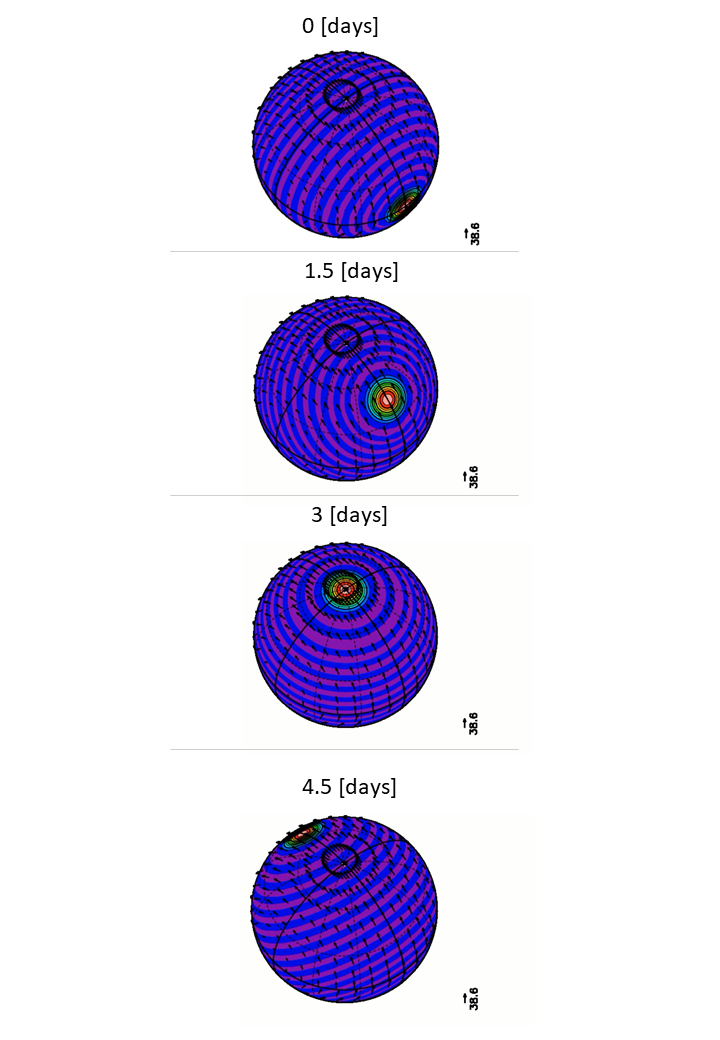
\includegraphics[clip,width=14cm]{./appendix/Williamson/fig/case1/case1_h.png}
 \end{center}
 \caption{\footnotesize{$BI=LLJQ0L$HB.EY%Y%/%H%k(B(T42, $BJBNs?t(B : ip = 2, $\alpha=\pi/2$).$B>e$+$i(B0$B!$(B1.5, 3, 4.5$BF|$N7W;;7k2L!%(B
$B0^EY(B$60^\circ$$B!$7PEY(B$230^\circ$$B$+$i8+$?5eLLEj1F(B.
}
}
 \label{case1_h}
\end{figure}
\clearpage
%
\begin{figure}[ht]
 \begin{center}
 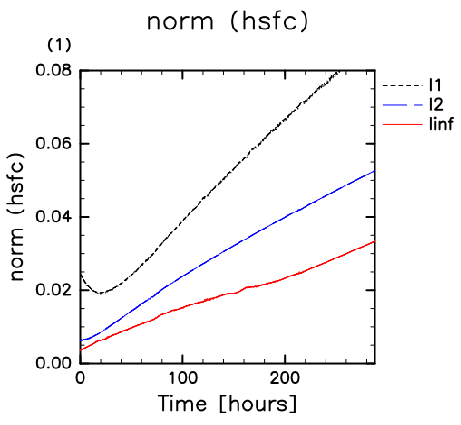
\includegraphics[clip,width=8cm]{./appendix/Williamson/fig/case1/case1_lh.png}
 \end{center}
 \caption{\footnotesize{$BI=LLJQ0L$NA45e8m:9(B(T42, $\alpha=\pi/2 -0.05 $)$B!%(B$l_1$ $B$O9u@~!$(B$l_2$ $B$O@D@~!$(B$l_\infty$ $B$O@V@~!%(B
2, 4, 8, 16 $BJBNs$N7W;;7k2L!%(B
}
}
 \label{case1_lh}
\end{figure}
%
\begin{figure}[ht]
 \begin{center}
 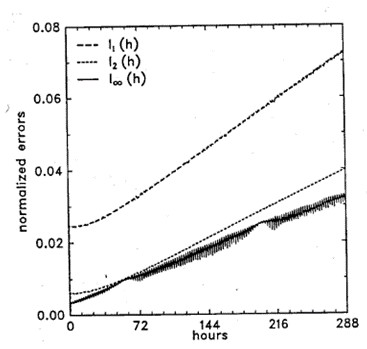
\includegraphics[clip,width=7cm]{./appendix/Williamson/fig/case1/case1_Jakob.jpg}
 \end{center}
 \caption{\footnotesize{$BI=LLJQ0L$NA45e8m:9(B(T42, $\alpha=\pi/2 -0.05 $)$B!%(B$l_1$ $B$OGK@~!$(B$l_2$ $B$OE@@~!$(B$l_\infty$ $B$O<B@~!%(B\cite{Jakob1993} $B?^(B1.3 $B$h$j0zMQ!%(B
}
}
 \label{case1_Jakob}
\end{figure}
\clearpage

%%%% case2 %%%%
%
\subsection{$B%F%9%H%1!<%9(B2 : $BDj>o$JHs@~7ABS>uCO9UN.(B}
$B$3$N%1!<%9$OHs@~7A5eLL@u?eJ}Dx<07O$NDj>o2r$H$7$FF@$i$l$k(B
$B9dBN2sE>$NN.$l>l$H!$$=$l$KCO9UN.J?9U$9$kI=LLJQ0L$NJ,I[$r=i4|$KM?$($k!%(B
$u, v$$B$N=i4|CM$O(B
\begin{align}
u&=u_0(\cos \theta \cos \alpha + \cos \lambda \sin \theta \sin \alpha), \\
v&=-u_0 \sin \lambda \sin \alpha.
\end{align}
$BN.@~4X?t$HB.EY%]%F%s%7%c%k$O(B
\begin{align}
\psi &= -a u_0 (\sin \theta \cos \alpha - \cos \lambda \cos \theta \sin \alpha), \\
\chi &= 0.
\end{align}
$B@dBP12EY$O(B
\begin{align}
\eta = \left (\frac{2u_0}{a}+ 2\Omega \right)(-\cos \lambda \cos \theta \sin \alpha + \sin \theta \cos \alpha).
\end{align}
$B2r@OE*$J9bEY>l$O(B
\begin{align}
gh = gh_0 - \left (a \Omega u_0 +\frac{u_0^2}{2} \right)(-\cos \lambda \cos \theta \sin \alpha + \sin \theta \cos \alpha)^2.
\end{align}
$B%3%j%*%j%Q%i%a!<%?$O(B
\begin{align}
f=2\Omega (-\cos \lambda \cos \theta \sin \alpha + \sin \theta \cos \alpha).
\end{align}
$B;HMQ$9$k%Q%i%a!<%?$O%1!<%9(B1$B$HF1MM$N(B$u_0=2\pi a /(12 \rm{~days})$$B!$$=$7$F(B$gh_0=2.94\times 10^4 ~\rm{m^2/s^2}$$B$r;HMQ$9$k!%(B

$BI=LLJQ0L$N7W;;7k2L$r?^(B\ref{case2_h}$B$K<($9!%(B
%
$B<0(B(\ref{linfh}) $B$NI=LLJQ0L$NA45e8m:9(B$l_\infty$$B$r?^(B\ref{case2_lh} $B$K<($9!%(B
$B?^(B\ref{case2_Jakob} $B$O$3$N%F%9%H%1!<%9$N7W;;$r9T$C$?(B\cite{Jakob1993}$B$N7W;;7k2L$G$"$k!%(B
\cite{Jakob1993} $B$KHf$Y$F8m:9$,Bg$-$$$,!$7W;;$K1F6A$,$"$k$h$&$J8m:9$O8+$i$l$J$$!%(B
%
%
\begin{figure}[ht]
 \begin{center}
 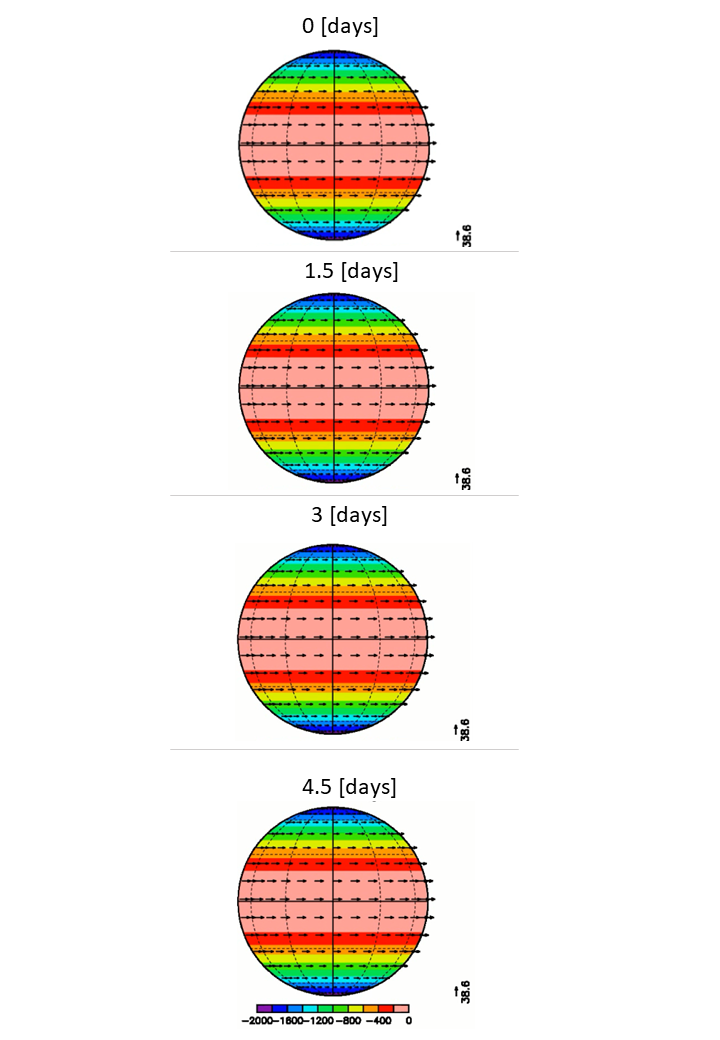
\includegraphics[clip,width=14cm]{./appendix/Williamson/fig/case2/case2_h.png}
 \end{center}
 \caption{\footnotesize{$BI=LLJQ0L$HB.EY%Y%/%H%k(B(T42, $BJBNs?t(B : ip = 2, $\alpha=\pi/2$).$B>e$+$i(B0$B!$(B1.5, 3, 4.5$BF|$N7W;;7k2L!%(B
$B0^EY(B$0^\circ$$B!$7PEY(B$0^\circ$$B$+$i8+$?5eLLEj1F(B.
}
}
 \label{case2_h}
\end{figure}
\clearpage
%
\begin{figure}[ht]
 \begin{center}
 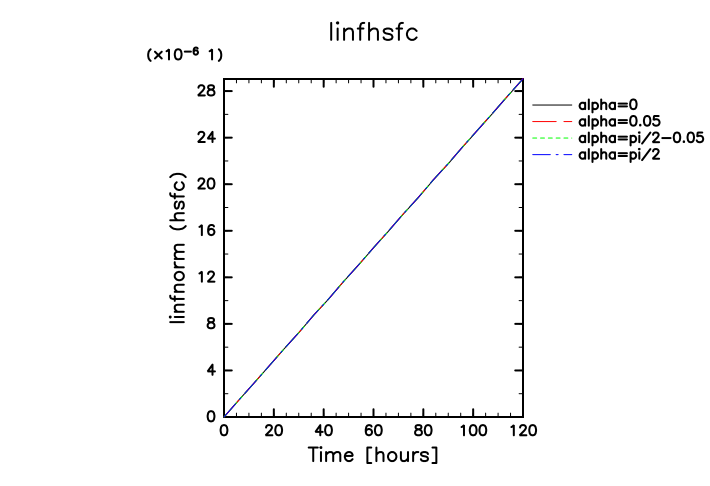
\includegraphics[clip,width=12cm]{./appendix/Williamson/fig/case2/case2_lh.png}
 \end{center}
 \caption{\footnotesize{$BI=LLJQ0L$N(B$l_\infty$ (T42)$B!%(B$\alpha = 0$ $B$O9u@~!$(B$\alpha = 0.05 $ $B$O@V@~!$(B
$\alpha = \pi/2 - 0.05 $ $B$ONP@~!$(B
$\alpha = \pi/2$ $B$O@D@~!%(B
}
}
 \label{case2_lh}
\end{figure}
%
\begin{figure}[ht]
 \begin{center}
 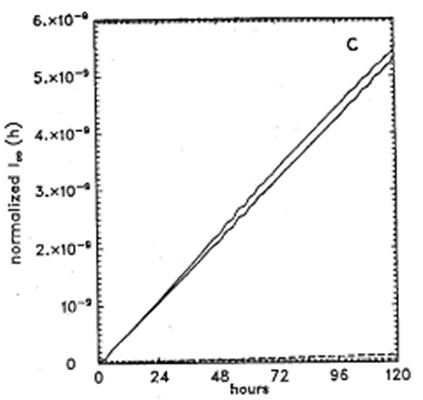
\includegraphics[clip,width=7cm]{./appendix/Williamson/fig/case2/case2_Jakob.jpg}
 \end{center}
 \caption{\footnotesize{$BI=LLJQ0L$N(B$l_\infty$ (T42)$B!%(B$\alpha = 0$ $B$OB@$$<B@~!$(B$\alpha = 0.05 $ $B$O:Y$$<B@~!$(B
$\alpha = \pi/2 - 0.05 $ $B$O:Y$$GK@~!$(B
$\alpha = \pi/2$ $B$OB@$$GK@~$H5-:\$7$F$"$C$?$,!$$I$N@~$,BP1~$9$k$N$+$o$+$i$J$+$C$?!%(B
\cite{Jakob1993} $B?^(B2.1 $B$h$j0zMQ!%(B
}
}
 \label{case2_Jakob}
\end{figure}
\clearpage
\subsubsection{SPMODEL ver.1, ver.2 $B$NJBNs2=8zN($NHf3S(B}
%
$B7W;;$K;HMQ$7$?(BCPU $B$O(BIntel(R) Core(TM) i7-9700K CPU @ 3.60GHz $B$G$"$k!%(B
ver.1 $B$H(Bver.2 $B$N<B9T;~4V$r?^(B\ref{para_1}$B$K<($9!%(B
8$BJBNs$N<B9T$,0lHV$O$d$/$J$k!%(B
$B$5$i$KJBNs?t$rA}$d$9$H<B9T;~4V$,D9$/$J$k!%(B
$B$3$l$O!$%N!<%I4V$G$NDL?.$K$h$k;~4V$,1F6A$7$F$$$k$H9M$($i$l$k!%(B
%
$B$^$?!$(Bver.1 $B$KHf$Y!$(Bver.2 $B$,Ls(B4.6$BG\$O$d$/$J$k!%(B
ver.2 $B$G$O0^EYJ}8~$N3J;RE@$K2C$(!$%9%Z%/%H%k%G!<%?$,El@>GH?tJ}8~$KJ,3d$5$l!$(B
$B<B9T;~4V$,C;$/$J$k$H9M$($i$l$k!%(B
%
\begin{figure}[ht]
 \begin{center}
 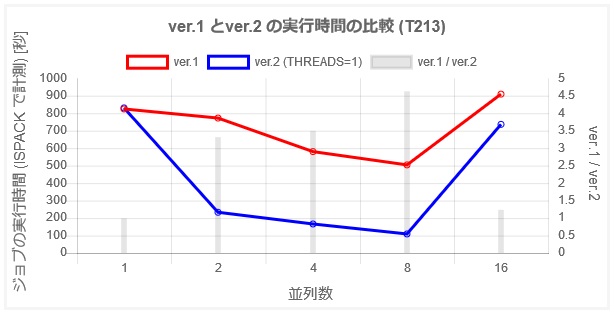
\includegraphics[clip,width=13cm]{./appendix/Williamson/fig/case2/parallel/p_1.png}
 \end{center}
 \caption{\footnotesize{ver.1 $B$H(Bver.2 $B$N<B9T;~4V$NHf3S(B(T213)$B!%:8(B : $B<B9T;~4V!%(Bver.1 $B$,@V@~!$(Bver.2 ($B%9%l%C%I?t$O(B1) $B$,@D@~!%(B
$B1&(B : ver.1 / ver.2 .
}
}
 \label{para_1}
\end{figure}
%
%%%% case3 %%%%
\newpage
\subsection{$B%F%9%H%1!<%9(B3 : $B6I:_$7$?Dj>oHs@~7ABS>uCO9UN.(B}
$B$3$N%1!<%9$O%1!<%9(B2$B$HF1MM!$Dj>o2r$H$7$FF@$i$l$kBS>u$JN.$l$rM?$($k$,!$(B
$B8B$i$l$?NN0h$G$N$_N.$l$,B8:_$9$k!%(B
%
$B$3$N%1!<%9$O$^$:<+E><4$H6K$,0lCW$9$k:BI87O(B$(\lambda', \theta')$\footnote{$B$D$^$j!$(B$\alpha=0$$B$N:BI87O!%(B}$B$G=q$-!$(B
$B<!$K%8%'%C%H$,:BI8@~$KJ?9T$G$O$J$$:BI87O(B$(\lambda, \theta)$$B$X!$3QEY(B$\alpha$$B$N2sE>$r9T$&$N$,$b$C$H$b4JC1$G$"$k!%(B
$BJQ49$9$kA0$N(B$(\lambda', \theta')$$B$NB.EY@.J,(B$(u', v')$$B$O(B
%
\begin{align}
u' &= u_0 b(x) b(x_e-x) e^{4/x_e}, \\
v' &=0.
\end{align}
$B$3$3$G!$(B
\begin{align}
b(x)= 
\begin{cases}
0 & x \le 0 \\
e^{-x^{-1}} & 0 < x, \notag
\end{cases}
\end{align}
\begin{align}
x=x_e(\theta'-\theta_b)(\theta_e-\theta_b)^{-1}.
\end{align}
$BN.@~4X?t$HB.EY%]%F%s%7%c%k$O(B
\begin{align}
\psi' &= -a \frac{\theta_e-\theta_b}{x_e}  u_0  e^{4/x_e} \int^x_{x_e} e^{-x_e/x'(x_e-x')} dx', \\
\chi' &=  0.
\end{align}
$u',v'$$B$+$i(B$u, v$$B$X$N$OJQ49$O0J2<$N$h$&$K9T$&!%$^$::BI8$O(B
\begin{align}
\sin \theta' &= \sin \theta \cos \alpha - \cos \theta \cos \lambda \sin \alpha, \\
\sin \lambda' \cos \theta' &= \sin \lambda \cos \theta.
\end{align}
$\lambda'$ $B$r7h$a$k:]$K$O(B
\begin{align}
\lambda' = 
\begin{cases}
\lambda'_p & \cos \alpha \cos \lambda \cos \theta + \sin \alpha \sin \theta \ge 0 \\
\pi - \lambda'_p & \cos \alpha \cos \lambda \cos \theta + \sin \alpha \sin \theta < 0. \notag
\end{cases}
\end{align}
$B$3$3$G!$(B$\lambda'_p$$B$O(B$\lambda$$B$N<gCM$G$"$k!%(B
$B%3%j%*%j%Q%i%a!<%?$O(B
\begin{align}
f &= 2\Omega(-\cos \lambda \cos \theta \sin \alpha + \sin \theta \cos \alpha)
\end{align}
$B$G$"$k!%$?$@$7!$JQ49A0$N:BI87O$G$O(B$f=2\Omega \sin {\theta'}$$B$G$"$k!%(B
%
\newpage
%
$BDj>o2r$N$?$a$K(B$h'$$B$O<!$N<0$rK~$?$5$J$1$l$P$J$i$J$$!%(B
\begin{align}
\frac{u'^2 \tan \theta'}{a} + \frac{g}{a} \DP{h'}{\theta'}+ fu'=0. \label{geobalance}
\end{align}
$B$3$l$O!$5eLL$G$N1?F0NLJ}Dx<0$N(B$v$$B@.J,$NCO9UN.J?9U$N4X78<0$+$iF@$i$l$k(B\footnote{
$B5eLL$G$N1?F0NLJ}Dx<0$N(B$v$$B@.J,$O(B
\begin{align}
\DP{v'}{t} + ( \Dvect{u'} \cdot \nabla)v + \left(f + \frac{u'}{a}\tan{\theta'} \right )u' + \frac{g}{a} \DP{h'}{\theta'}  = 0.
\end{align}
$BCO9UN.J?9U$N>uBV$r9M$($k$?$a!$;~4VJQ2=9`$H0\N.9`$rL5;k$9$k$H(B
\begin{align}
\frac{u'^2 \tan \theta'}{a} + \frac{g}{a} \DP{h'}{\theta'}+ fu'=0
\end{align}
$B$H$J$j!$<0(B(\ref{geobalance})$B$,F@$i$l$k!%(B
}$B!%(B
%
$h'$$B$O$3$N<0$r@QJ,$9$k$3$H$GF@$i$l(B
\begin{align}
h=h_0 - \frac{a}{g}\int^{\theta'}_{-\pi/2} \left (2\Omega \sin \tau + \frac{u'(\tau)\tan \tau}{a} \right)u'(\tau) d\tau
\end{align}
$B$H$J$k!%(B$h_0$$B$O%1!<%9(B2$B$HF1MM$K(B
$gh_0=2.94 \times 10^4 ~\rm{m^2/s^2}$$B$GM?$($i$l$k!%(B
$B%Q%i%a!<%?$O(B$u_0 = 2\pi a/ (12 {\rm{~days}}), \theta_b=-\pi/6, \theta_e = \pi/2, x_e = 0.3$$B$rMQ$$$k!%(B
%

$BI=LLJQ0L$N7W;;7k2L$r?^(B\ref{case3_h}$B$K<($9!%(B
%
$B<0(B(\ref{linfh}) $B$NI=LLJQ0L$NA45e8m:9(B$l_\infty$$B$r?^(B\ref{case3_lh} $B$K<($9!%(B
$B?^(B\ref{case3_Jakob} $B$O$3$N%F%9%H%1!<%9$N7W;;$r9T$C$?(B\cite{Jakob1993}$B$N7W;;7k2L$G$"$k!%(B
\cite{Jakob1993} $B$KHf$Y$F8m:9$,$+$J$jBg$-$$!%(B
$B8m:9$,Bg$-$$860x$H$7$F!$=i4|CM$KM?$($kI=LLJQ0L$rBf7A8x<0$rMQ$$$F!$(B
$B7W;;$7$?$,$=$N@:EY$,0-$$$3$H$,9M$($i$l$k!%(B
%
%
\begin{figure}[ht]
 \begin{center}
 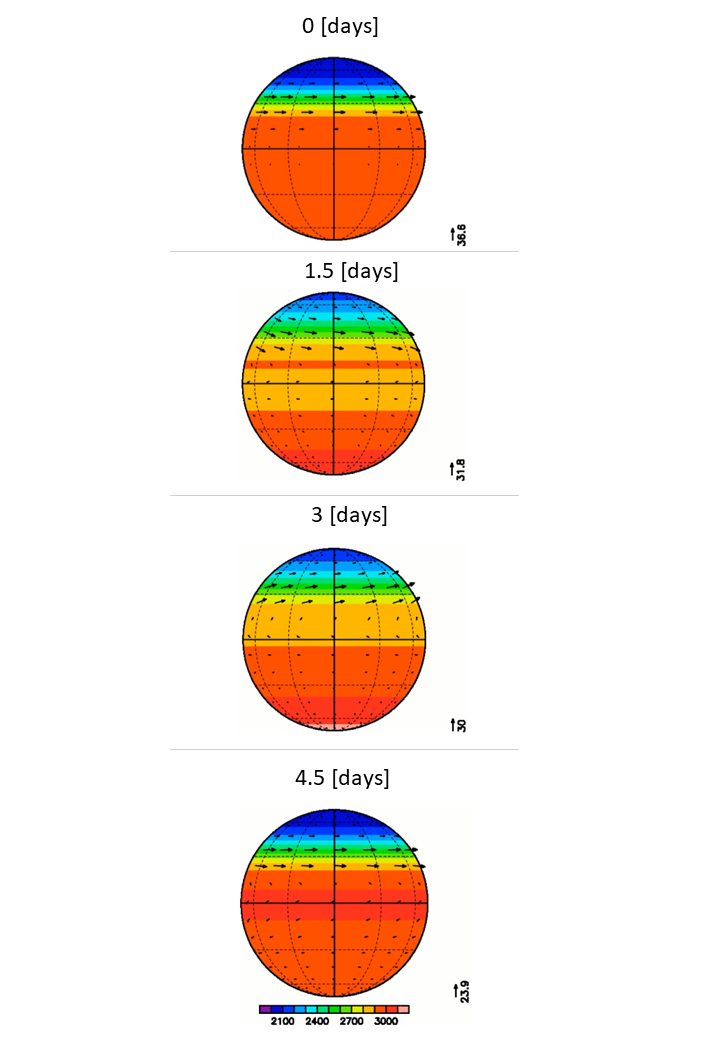
\includegraphics[clip,width=14cm]{./appendix/Williamson/fig/case3/case3_h.png}
 \end{center}
 \caption{\footnotesize{$BI=LLJQ0L$HB.EY%Y%/%H%k(B(T42, $BJBNs?t(B : ip = 2, $\alpha=\pi/2$).$B>e$+$i(B0$B!$(B1.5, 3, 4.5$BF|$N7W;;7k2L!%(B
$B0^EY(B$0^\circ$$B!$7PEY(B$0^\circ$$B$+$i8+$?5eLLEj1F(B.
}
}
 \label{case3_h}
\end{figure}
\clearpage
%
\begin{figure}[ht]
 \begin{center}
 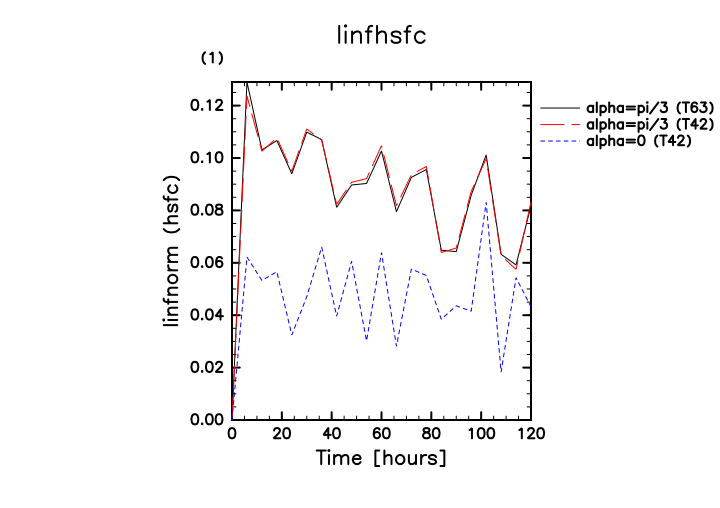
\includegraphics[clip,width=12cm]{./appendix/Williamson/fig/case3/case3_lh.png}
 \end{center}
 \caption{\footnotesize{$BI=LLJQ0L$N(B$l_\infty$ $B!%(B$\alpha = \pi/3$ (T63) $B$O9u@~!$(B$\alpha = \pi/3$ (T42) $B$O@V@~!$(B
$\alpha = 0$ (T42) $B$O@D@~!%(B
}
}
 \label{case3_lh}
\end{figure}
%
\begin{figure}[ht]
 \begin{center}
 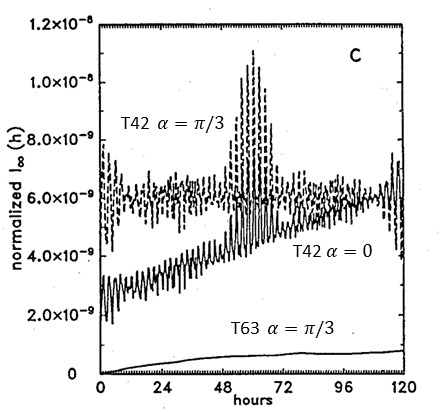
\includegraphics[clip,width=7cm]{./appendix/Williamson/fig/case3/case3_Jakob.jpg}
 \end{center}
 \caption{\footnotesize{$BI=LLJQ0L$N(B$l_\infty$ (T42)$B!%(B$\alpha = \pi/3$ (T63) $B$O:Y$$<B@~!$(B$\alpha = \pi/3$ (T42) $B$OE@@~!$(B
$\alpha = 0$ (T42)  $B$OB@$$<B@~!%(B
\cite{Jakob1993} $B?^(B3.1 $B$h$j0zMQ!%(B
}
}
 \label{case3_Jakob}
\end{figure}
\clearpage
%
%%%% case4 %%%%
\subsection{$B%F%9%H%1!<%9(B4 : $B0\F0$9$kDc5$05$r;}$D6/@)$5$l$?N.$l(B}
$B$3$N%1!<%9$O0\F0$9$kDc5$05$r$"$i$o$9<!$N6/@)9`$r2C$(!$(B
$BHs@~7AHsDj>oJ}Dx<0$KBP$9$kI>2A$r9T$&!%(B
$B6/@)9`$O(B
\begin{align}
F_u &= \DD{\tilde{u}}{t}-\frac{\tilde{u}\tilde{v}\tan \theta}{a}
+\frac{g}{a \cos \theta}\DP{\tilde{h}}{\lambda}-f\tilde{v}, \\
F_v &= \DD{\tilde{v}}{t}+\frac{\tilde{u}\tilde{u}\tan \theta}{a}
+\frac{g}{a}\DP{\tilde{h}}{\theta}+f\tilde{u}, \\
F_h &= \DD{\tilde{h}}{t} + \frac{\tilde{h}}{a \cos \theta}\left [\DP{\tilde{u}}{\lambda}+ \DP{\tilde{v}\cos \theta}{\theta} \right ]
\end{align}
$B$GM?$($i$l$k!%(B
$\tilde{u}, \tilde{v}, \tilde{h}$ $B$O(B
\begin{align}
\tilde{u} &= \bar{u} - \bar{\psi}_\theta, \\
\tilde{v} &= \frac{\bar{\psi}_\lambda}{a \cos \theta}, \\
g \tilde{h} &= g \bar{h} + f \bar{\psi},
\end{align}
$B$3$3$G!$(B
\begin{align}
\bar{u} &= u_0 \sin^{14} (2\theta), \\
g\bar{h} &= gh_0 - \int^\theta_{-\pi/2} [a f(\tau) + \bar{u}(\tau) \tan \tau] \bar{u}(\tau) d\tau, \\
\bar{\psi}(\lambda, \theta, t) &= \psi_0 e^{- \sigma ((1-C)/(1+C))}.
\end{align}
$\psi_0=-0.03(gh_0/f_0), \sigma=(12.74244)^2, gh_0=10^5 ~{\rm{m^2/s^2}}, f_0=2\Omega \sin(\pi/4)$$B$G$"$k!%(B$C$$B$O(B
\begin{align}
C= \sin \theta_0 \sin \theta + \cos \theta_0 \cos \theta \cos \left (\lambda - \frac{u_0}{a}t-\lambda_0 \right ).
\end{align}
$B=i4|$NDc5$05$NCf?4$O(B$(\lambda_0,\theta_0)=(0,\pi/4)$$B$K0LCV$7$F$$$k!%(B
$BN.@~4X?t$HB.EY%]%F%s%7%c%k$O(B
\begin{align}
\psi(\lambda, \theta, t) &= - \int^\theta_{-\pi/2} a\bar{u}(\tau)d\tau + \bar{\psi}(\lambda, \theta, t), \\
\chi &= 0.
\end{align}

$BI=LLJQ0L$N2r@O2r$H7W;;7k2L$r?^(B\ref{case4_h}$B$K<($9!%(B
$B7W;;7k2L$G$O2r@O2r$H$O0c$$!$6/@)$H$7$FM?$($F$$$k(B
$BDc5$05$NCM$,;~4V$H$H$b$K>.$5$/$J$C$F$7$^$&!%(B
$BB.EY>l$bDc5$05$N<~$j$G!$2r@O2r$H0[$J$C$F$$$k!%(B
%
$B$^$?!$<0(B(\ref{linfh}) $B$NI=LLJQ0L$NA45e8m:9(B$l_\infty$$B$r?^(B\ref{case4_lh} $B$K<($9!%(B
$B?^(B\ref{case4_Jakob} $B$O$3$N%F%9%H%1!<%9$N7W;;$r9T$C$?(B\cite{Jakob1993}$B$N7W;;7k2L$G$"$k!%(B
\cite{Jakob1993} $B$KHf$Y$F8m:9$,$+$J$jBg$-$$!%(B
$B8m:9$,Bg$-$$860x$H$7$F!$%1!<%9(B3 $B$HF1MM!$I=LLJQ0L$N@QJ,$r7W;;$9$kI,MW$,$"$j!$(B
$B$=$N1F6A$,9M$($i$l$k!%(B
$B$^$?!$6/@)9`$NM?$(J}!$%3!<%I$N5-=R$N;EJ}$r3N$+$a$kI,MW$,$"$k!%(B
%
%
\begin{figure}[ht]
 \begin{center}
 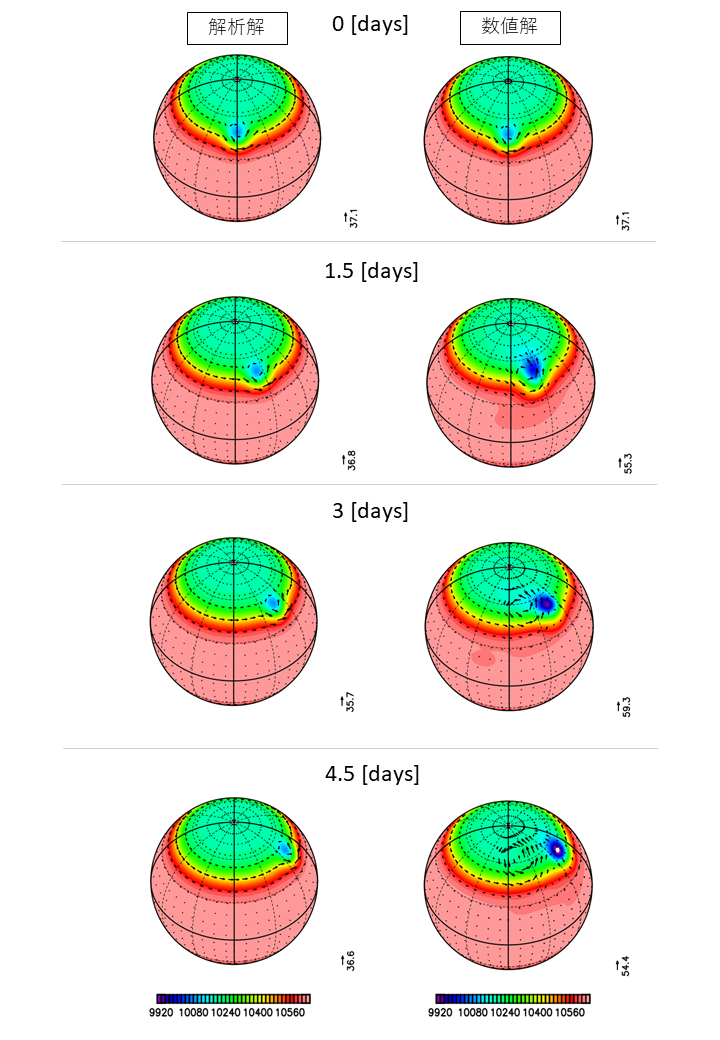
\includegraphics[clip,width=14cm]{./appendix/Williamson/fig/case4/case4_h.png}
 \end{center}
 \caption{\footnotesize{$BI=LLJQ0L$HB.EY%Y%/%H%k(B(T42, $BJBNs?t(B : ip = 2, $u_0 = 20 $~m/s).
$B:8(B $B!'2r@O2r!$1&(B : $B?tCM2r(B.
$B>e$+$i(B0$B!$(B1.5, 3, 4.5$BF|$N7W;;7k2L!%(B
$B0^EY(B$0^\circ$$B!$7PEY(B$45^\circ$$B$+$i8+$?5eLLEj1F(B.
}
}
 \label{case4_h}
\end{figure}
\clearpage
%
\begin{figure}[ht]
 \begin{center}
 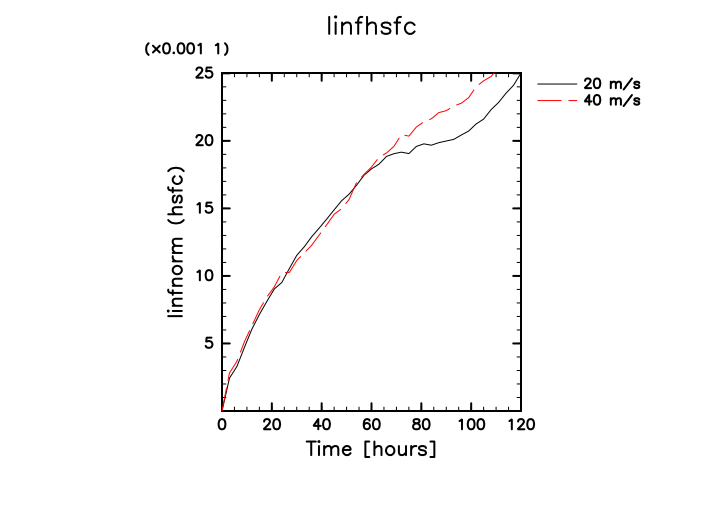
\includegraphics[clip,width=12cm]{./appendix/Williamson/fig/case4/case4_lh.png}
 \end{center}
 \caption{\footnotesize{$BI=LLJQ0L$N(B$l_\infty$ (T42)$B!%(B$u_0 = 20$~m/s $B$O9u@~!$(B$u_0 = 40$~m/s $B$O@V@~!%(B
}
}
 \label{case4_lh}
\end{figure}
%
\begin{figure}[ht]
 \begin{center}
 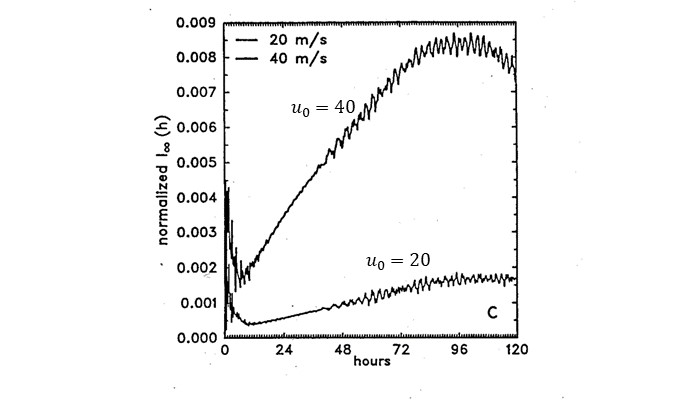
\includegraphics[clip,width=12cm]{./appendix/Williamson/fig/case4/case4_Jakob.jpg}
 \end{center}
 \caption{\footnotesize{$BI=LLJQ0L$N(B$l_\infty$ (T42)$B!%(B$u_0 = 20$~m/s $B$O:Y$$<B@~!$(B$u_0 = 40$~m/s $B$OB@$$<B@~!%(B
\cite{Jakob1993} $B?^(B4.6 $B$h$j0zMQ!%(B
}
}
 \label{case4_Jakob}
\end{figure}
\clearpage
%
%%%% case5 %%%%
\subsection{$B%F%9%H%1!<%9(B5 : $B8IN)$7$?;3$r1[$($kBS>uN.(B}
$B$3$N%1!<%9$OCf0^EY$K8IN)$7$?;3$rCV$-!$(B
$B$=$l$K$h$kN.BN$N1~Ez$rD4$Y$k$b$N$G$"$k!%(B
$B=i4|$NB.EY>l$HI=LLJQ0L$O%1!<%9(B2$B$H(B
$BF1MM$G!$BS>uN.$,8IN)$7$?;3$K>WFM$7$F$$$k!%(B
$B;3$N9b$5(B$h_s$$B$O(B
\begin{align}
h_s = h_{s0} (1-r/R).
\end{align}
$B$3$3$G!$(B$h_{s0}=2000 ~$m$B!$(B$R=\pi/9, r^2= {\rm{min}}[R^2, (\lambda-\lambda_c)^2 + (\theta-\theta_c)^2]$$B$G$"$k!%(B
\\
\quad
$B;3$NCf?4$O(B$\lambda_c=3\pi/2$B!$(B~\theta_c=\pi/6$$B$H$9$k!%(B
$B$3$N%1!<%9$O2r@O2r$,CN$i$l$F$$$J$$$N$G!$J]B8NL$r3NG'$9$k!%(B
$B$"$kJ]B8NL(B$\xi$$B$rMQ$$$F!$@55,2=$7$?J]B8NL(B$I_i(\xi)$$B$O(B
\begin{equation}
I_i(\xi(t)=\frac{I[\xi(\lambda,\theta,t)]-I[\xi(\lambda,\theta,0)]}{I[\xi(\lambda,\theta,0)]}. 
\end{equation}
$B$3$3$G!$(B$I$$B$O<0(B(\ref{eq:I})$B$GDj5A$5$l$?$b$N$G$"$k!%J]B8NL$O(B
\\$B<ANL(B($i=1$)
\begin{equation}
\xi=h^*
\end{equation}
$BA4%(%M%k%.!<(B($i=2$)
\begin{equation}
\xi=\frac{1}{2}h^* \Dvect{u}^2 + \frac{1}{2}g(h^2-h^2_s)
\end{equation}
$B%]%F%s%7%c%k%(%s%9%H%m%U%#!<(B($i=3$)
\begin{equation}
\xi=0.5(\zeta+f)^2/h^*
\end{equation}
$B$G$"$k!%$3$3$G!$(B$h^*$$B$ON.BNAX$N8|$5$G$"$k(B\footnote{$B<+M3I=LL(B$h$$B$O(B$h=h^*+h_s$$B$G=q$+$l$k!%(B}$B!%(B
$B12EY$HH/;6$O=i4|CM$,(B0$B$J$N$GHs@55,2=@QJ,$G$"$k0J2<$r<($9I,MW$,$"$k!%(B
\\$B12EY(B($i=4$)
\begin{equation}
\xi=\zeta
\end{equation}
$BH/;6(B($i=5$)
\begin{equation}
\xi=\delta.
\end{equation}

%%%% case6 %%%%
\subsection{$B%F%9%H%1!<%9(B6 : $B%m%9%S!<%O%&%k%t%#%C%DGH(B}


%
\newpage
%
%%  Fig  %%
\def\apetitleFig{: 実験図集}
\def\apeFig{\Alph{section} \apetitleFig}
\section{\apetitleFig}
\label{ape:Fig}
\markright{\apeFig}
%% Appendix C %%
%%%%%%%%%%%%%%%%
\setcounter{subsection}{0}
\setcounter{subsubsection}{0}
\setcounter{figure}{0}
\setcounter{table}{0}
\setcounter{equation}{0}
\setcounter{secnumdepth}{3}
\renewcommand{\thesubsection}{\Alph{section}.\arabic{subsection}} 
\renewcommand{\thesubsubsection}{\Alph{section}.\arabic{subsection}.\arabic{subsubsection}} 
\renewcommand{\thefigure}{\Alph{section}.\arabic{subsection}.\arabic{figure}}
\renewcommand{\thetable}{\Alph{section}.\arabic{subsection}.\arabic{table}}
%
\subsection{$B<B83(B1}
$B<B83(B1$B$G$O(B$g'h_{\rm{eq}}$$B$rJQ2=$5$;$?<B83$r9T$&!%(B
$BMQ$$$?%Q%i%a!<%?$OI=(B\ref{table2}$B$r;2>H!%(B

%
\subsubsection{A1 : $g'h_{\rm{eq}} = 6 \times 10^4 \rm{~m^2 \cdot s^{-3}}$}
\begin{figure}[ht]
 \begin{center}
 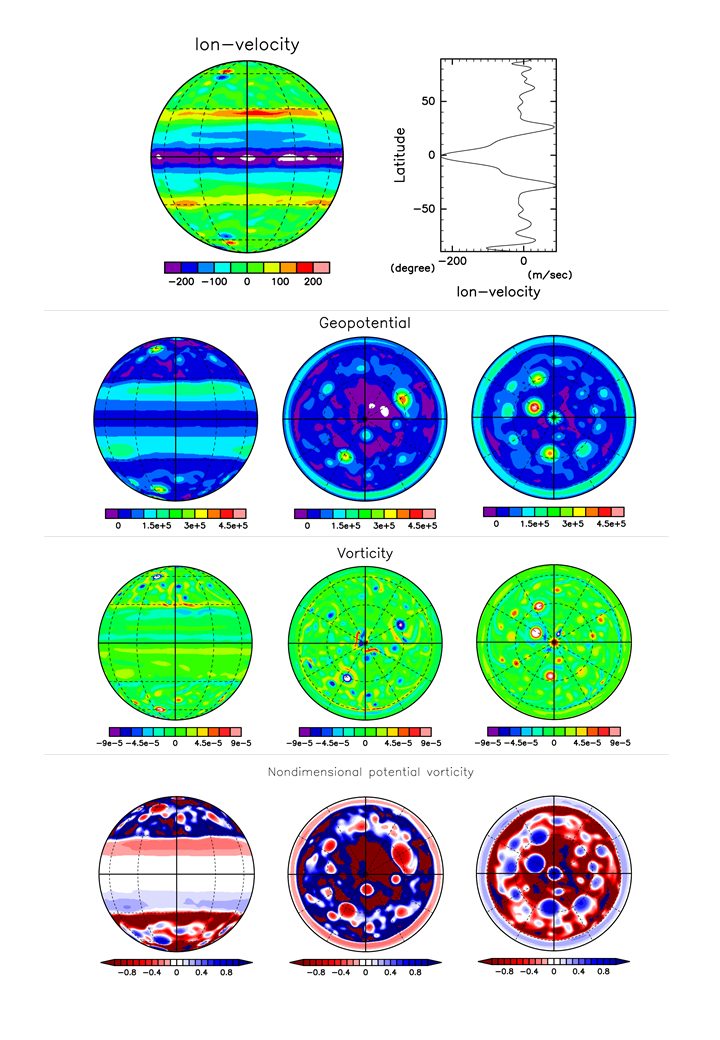
\includegraphics[clip,width=11cm]{./appendix/C/fig_colle/case1/a1_13/1.png}
 \end{center}
 \caption{\footnotesize{ 
}
}
 \label{fig:a1_13_1}
\end{figure}

\begin{figure}[ht]
 \begin{center}
 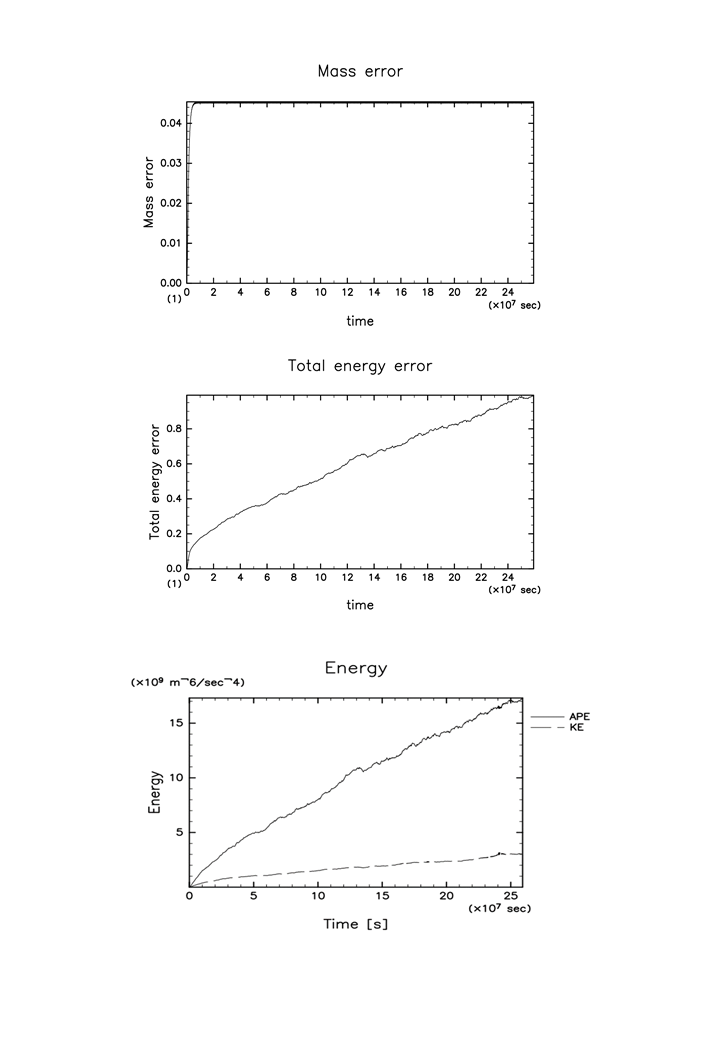
\includegraphics[clip,width=14cm]{./appendix/C/fig_colle/case1/a1_13/2.png}
 \end{center}
 \caption{\footnotesize{
}
}
 \label{fig:a1_13_2}
\end{figure}


%%%%%%%%%%%%%%%%
\def\acknow{謝辞}
\chapter*{\acknow}
\addcontentsline{toc}{chapter}{\acknow}
\label{acknow}
\markright{謝辞}
ddd

\newpage
\renewcommand{\bibname}{参考文献}
\addcontentsline{toc}{chapter}{参考文献}
\bibliographystyle{abbrvnat}
\nocite{*}
\markright{参考文献}
\bibliography{./reference/reference}

\end{document}
